%!TEX root = ../MainBody.tex

% 第二章
% ═══════════════════════════════════════════════════════════════════
% 写作思路（全章概要）：
%   本章是全文的理论根基，为第三~五章提供必要的知识铺垫。
%   与第一章文献综述的区别：第一章侧重"评述"（谁做了什么、各方法优劣），
%   本章侧重"阐述"（读者需要理解的具体理论和技术细节）。
%
%   每一节对应后续一章的理论基础：
%     2.1 热输运理论      → 支撑第三章求解器的物理模型
%     2.2 蒙特卡洛方法    → 支撑第三章求解器的数值方法
%     2.3 光追加速技术    → 支撑第四章 OptiX 后端
%     2.4 Wavefront 模型  → 支撑第三章并行化改造
% ═══════════════════════════════════════════════════════════════════
\chapter{相关理论与技术介绍}

\section{热输运理论}
%% [篇幅需求] 约1500字，重在建立物理直觉与数学符号约定，为后续蒙特卡洛求解铺垫。
%% [写作总思路]
%%   先分述三种基本热传递机制（各有独立小节），再集中讨论多机制耦合问题，
%%   最后以"现有数值方法难以高效耦合求解"作为动机，自然引出蒙特卡洛路径追踪统一框架。
%%   三种机制的篇幅按其在本文中的建模深度分配：传导 > 辐射 > 对流（对流建模最少，一段带过）。

\subsection{热传导}
%% 写作思路：
%%   - 物理机制：微观声子/自由电子碰撞传能，宏观上服从局域热平衡假设。
%%   - 傅里叶定律（本构关系）：$\mathbf{q} = -\lambda \nabla T$，说明各符号含义及导热系数 $\lambda$ 的各向同性假设。
%%   - 能量守恒推导热传导方程：$\rho c_p \frac{\partial T}{\partial t} = \nabla \cdot (\lambda \nabla T) + \dot{S}$，指出体积热源项 $\dot{S}$（辐射吸收在此处的耦合角色）。
%%   - 边界条件类型：Dirichlet（给定温度）、Neumann（给定热流）、Robin（辐射/对流混合边界）。
%%   - 【重点强调】在耦合热输运求解中，热传导是三种机制中最复杂、计算开销最大的部分，其主导地位体现在：
%%       (1) 偏微分方程维度高：热传导方程是三维抛物型 PDE，求解域为固体体积，而辐射仅涉及表面积分。
%%       (2) 蒙特卡洛求解代价高：基于随机游走（Brownian motion）的蒙特卡洛传导求解需大量短步长
%%           游走样本（步长与材料热扩散率、时间步相关），每步均需一次几何相交查询（判断是否撞到
%%           固体边界或进入不同材质区域），路径样本数远超其他路径。
%%       (3) 温度场更新瓶颈：整个求解迭代的收敛速度受制于固体内温度场的热传导弛豫时间，
%%           而非辐射或对流的边界交换速率。
%%     因此，加速几何相交查询对整体求解性能具有决定性作用，这也是本文引入 GPU 硬件光追的
%%     核心动机之一（详见第四章）。
%% [公式需求] 傅里叶定律、热传导方程（含时间项与稳态简化形式）
%% [引用需求] \cite{bergmanFundamentalsHeatMass2011}

热传导是固体介质中热量传递的基本方式。在微观层面，热传导依赖声子碰撞（非金属）和自由电子迁移（金属导体）实现能量转移；在宏观层面，当材料满足局域热平衡假设时，热流密度与温度梯度的关系由傅里叶定律（Fourier's Law）表达：
\begin{equation}
    \mathbf{q} = -\lambda \nabla T
    \label{eq:fourier}
\end{equation}
其中 $\mathbf{q}$（W/m²）为热流密度矢量，$\lambda$（W/(m·K)）为导热系数，$T$（K）为温度场。负号指出热量沿温度降低方向传递。对于各向同性均质材料，$\lambda$ 为标量；对于各向异性材质（如复合材料、晶体），则退化为二阶张量。

将傅里叶定律代入能量守恒方程，可推导出热传导方程：
\begin{equation}
    \rho c_p \frac{\partial T}{\partial t} = \nabla \cdot (\lambda \nabla T) + \dot{S}
    \label{eq:heat_conduction}
\end{equation}
其中 $\rho$（kg/m³）为材料密度，$c_p$（J/(kg·K)）为比热容，$\dot{S}$（W/m³）为体积热源项。在耦合热输运场景中，$\dot{S}$ 包含辐射被固体吸收所转化的热源及其他内热源。对稳态问题，方程左端时间导数项为零，退化为泊松方程 $\nabla \cdot (\lambda \nabla T) + \dot{S} = 0$。

热传导方程的求解需配合以下边界条件之一：
\begin{itemize}
    \item 第一类（Dirichlet）边界：直接给定边界温度 $T|_{\partial\Omega} = T_w$，例如固体壁面与恒温热源直接接触，壁面温度由热源温度直接确定。
    \item 第二类（Neumann）边界：给定法向热流 $-\lambda \nabla T \cdot \hat{n}|_{\partial\Omega} = q_w$，例如绝热边界（$q_w = 0$，无热流穿过）或已知外加热流密度的加热面。
    \item 第三类（Robin）边界：联立温度与热流，典型形式为辐射-对流混合边界条件，例如固体外壁面同时受到对流冷却与辐射散热，热流由表面温度通过换热系数和 Stefan-Boltzmann 定律共同确定。
\end{itemize}

在本文的耦合热输运求解框架中，热传导是三种机制中计算开销最大、地位最为核心的部分，这一主导性体现在三个层面：其一，热传导方程是三维抛物型偏微分方程，求解域为整个固体体积，而热辐射仅涉及表面积分，体积求解的空间维度远高于后者；其二，在蒙特卡洛路径追踪框架中（详见第 2.2 节），传导路径通过三维布朗随机游走逼近，需要大量短步长采样，每步均需一次几何相交查询以判断游走粒子是否触及固体边界或跨越材质界面，路径样本总量远超辐射路径；其三，耦合迭代的整体收敛速度受制于固体温度场的热传导弛豫时间常数，而非辐射或对流的边界交换速率。上述特点决定了：大批量几何相交查询的吞吐能力是制约整体仿真性能的关键瓶颈，这也构成了本文引入 GPU 硬件光线追踪加速的核心动机之一。

\subsection{热辐射}
%% 写作思路：
%%   - 物理机制：电磁波辐射传能，不需要介质接触，是红外仿真的主导机制。
%%   - 黑体辐射基础：普朗克分布、Stefan-Boltzmann 定律 $E_b = \sigma T^4$、Kirchhoff 定律（发射率=吸收率）。
%%   - 辐射传输方程（RTE）：沿射线方向 $\hat{\omega}$ 的强度变化，含自发发射、吸收、散射项：
%%         $\hat{\omega} \cdot \nabla L = \kappa (L_b - L) - \sigma_s L + \frac{\sigma_s}{4\pi} \int_{4\pi} L(\hat{\omega}') \, d\hat{\omega}'$
%%   - 实际工程场景：表面辐射（漫射灰体假设）是本文主要考虑的情形，介质散射暂不讨论。
%% [公式需求] Stefan-Boltzmann 定律、Kirchhoff 定律、辐射传输方程 (RTE) 微分形式
%% [引用需求] \cite{modestRadiativeHeatTransfer2013,howellThermalRadiationHeat2021}

热辐射以电磁波形式传递能量，无需介质接触即可在真空中远距离传播，是红外仿真场景中的重要传热机制。理想黑体是最完美的辐射源，其半球辐射力由 Stefan-Boltzmann 定律给出：
\begin{equation}
    E_b = \sigma T^4
\end{equation}
其中 $\sigma = 5.67 \times 10^{-8}$ W/(m²·K$^4$) 为 Stefan-Boltzmann 常数。实际工程材料为灰体，辐射力通过发射率 $\varepsilon \in [0,1]$ 修正为 $E = \varepsilon \sigma T^4$。根据 Kirchhoff 定律，在热平衡条件下材料的光谱发射率等于光谱吸收率（$\varepsilon_\lambda = \alpha_\lambda$），这为仿真中材料参数的统一描述提供了依据。

在参与性介质中，辐射强度 $L$（W/(m²·sr)）沿传播方向 $\hat{\omega}$ 的变化由辐射传输方程（Radiative Transfer Equation，RTE）描述：
\begin{equation}
    \hat{\omega} \cdot \nabla L(\mathbf{x}, \hat{\omega})
    = \kappa\bigl[L_b(T) - L(\mathbf{x}, \hat{\omega})\bigr]
    - \sigma_s L(\mathbf{x}, \hat{\omega})
    + \frac{\sigma_s}{4\pi} \int_{4\pi} L(\mathbf{x}, \hat{\omega}') \, \mathrm{d}\hat{\omega}'
    \label{eq:rte}
\end{equation}
其中 $\kappa$（m$^{-1}$）为吸收系数，$\sigma_s$（m$^{-1}$）为散射系数，$L_b(T) = \sigma T^4/\pi$ 为黑体辐射强度。方程右侧三项依次对应热发射引起的强度增益、出散射引起的强度衰减，以及来自其他方向的入散射能量补偿。

本文聚焦于不透明固体表面之间的辐射换热，采用漫射灰体（diffuse-gray）假设：表面辐射各向同性，材料发射率与波长无关。在此简化下，固体间介质视为透明（$\kappa = \sigma_s = 0$），RTE 退化为纯直线传播问题——辐射强度在两次表面碰撞之间沿直线保持不变，辐射传输仅需追踪光线的几何可见性。这一特性使光线追踪成为求解此类辐射传输的天然工具。此处，$\kappa > 0$ 或 $\sigma_s > 0$ 的介质称为参与性介质（participating media），其对立面即为上述透明介质假设。

表面辐射特性的完整描述采用双向反射分布函数（Bidirectional Reflectance Distribution Function，BRDF）$f_r(\hat\omega_i, \hat\omega_o) = \mathrm{d}L_o(\hat\omega_o) / \mathrm{d}E_i(\hat\omega_i)$（单位 sr$^{-1}$），定义为出射辐射亮度与入射辐照度之比\cite{modestRadiativeHeatTransfer2013,howellThermalRadiationHeat2021}。工程热辐射中最常用的简化模型为Lambert（漫射）反射，此时 $f_r = \rho_d / \pi$，$\rho_d = 1 - \varepsilon$ 为漫反射率。本文与 Bati 等人\cite{batiCouplingConductionConvection2023}相同，采用 Lambert 反射模型。

\subsection{热对流}
%% 写作思路（篇幅精简，约100字正文）：
%%   - 简述物理机制：流体宏观运动携带热量，固-流界面产生对流换热。
%%   - 牛顿冷却定律：$q = h(T_s - T_\infty)$，对流换热系数 $h$ 是综合了流场信息的集总参数。
%%   - 直接说明本文的建模立场：本文不求解 Navier-Stokes 方程，对流仅作为边界条件（CNV 过程）
%%     出现——给定预计算或用户指定的 $h$ 值，在固体表面施加对流热损失。
%%     这是工程热仿真中的标准解耦简化，将对流的复杂流场问题与热传导/辐射求解解耦，
%%     不影响本文所关注的辐射传热建模精度。
%% [公式需求] 牛顿冷却定律（一行即可）
%% [引用需求] \cite{bergmanFundamentalsHeatMass2011}

热对流通过流体的宏观运动携带热量，是固体壁面与流体环境之间重要的热交换方式。固-流界面处的对流换热通常以牛顿冷却定律（Newton's Law of Cooling）建模：
\begin{equation}
    q_\mathrm{conv} = h\,(T_s - T_\infty)
\end{equation}
其中 $q_\mathrm{conv}$（W/m²）为对流热流密度，$T_s$ 与 $T_\infty$ 分别为固体表面温度和远场流体温度，$h$（W/(m²·K)）为对流换热系数，综合了边界层厚度、流速、流体热物性等流场信息。

本文不求解 Navier-Stokes 方程，对流以简化的边界条件（CNV 过程）形式参与耦合求解：对流换热系数 $h$ 是一个场景相关的自定义常量，在固体表面施加对应的热损失约束\cite{bergmanFundamentalsHeatMass2011}。Bati 等人\cite{batiCouplingConductionConvection2023}的耦合框架同样采用此简化——将对流以 Newton 冷却定律形式纳入边界条件，$h$ 为用户输入的经验参数。

$h = \text{const}$ 假设的适用性可通过 Biot 数 $\text{Bi} = hL_c/k$ 评估，其中 $L_c$ 为固体特征长度、$k$ 为固体导热系数。当 $\text{Bi} \ll 1$ 时，固体内部温度梯度远小于固-流界面温差，表面温度近似均匀，恒定 $h$ 即可充分描述对流热交换\cite{bergmanFundamentalsHeatMass2011}。该条件在薄壁高导热金属结构（如铝合金薄板、散热翅片）中广泛成立。对于 $\text{Bi} \gg 1$ 的场景（厚壁低导热体或高速气流），$h$ 的空间变化不可忽略，需引入局部 $h(\mathbf{x})$ 分布或直接耦合 CFD 流场求解。本文验证场景均满足 $\text{Bi} < 0.1$ 的集总参数适用条件。

这是工程热仿真中标准的解耦简化策略，适用于强制对流或已知经验关联式的场景；对于自然对流或强烈耦合的流-热问题，则需要 Navier-Stokes 方程的完整求解。

\subsection{多机制耦合热输运}
%% 写作思路：
%%   - 说明三种机制在实际工程场景（如飞行器舱体热防护、红外特征预测）中同时存在，不可单独求解。
%%   - 耦合形式：
%%       (a) 边界耦合：固-流-辐射三者联立的能量平衡边界条件（表面温度由三者共同决定）：
%%             $-\lambda \nabla T \cdot \hat{n} + h(T_s - T_\infty) + \varepsilon \sigma T_s^4 - \alpha G = 0$
%%       (b) 体积耦合：半透明介质中辐射吸收项 $\dot{S}$ 直接作为热传导方程的体热源。
%%   - 耦合带来的数值挑战：非线性（$T^4$ 项）、各机制时间尺度差异大、分区网格难以统一。
%%   - 引出动机：本文采用蒙特卡洛路径追踪在统一的路径空间中描述三种机制，自然处理耦合边界，
%%     避免了传统方法的跨模块耦合迭代。
%%   - 引出 GPU 加速动机（此处埋伏笔，2.3~2.4 展开）：三种机制统一在同一路径空间后，
%%     所有过程（RAD/BND/CND/CNV）大量依赖几何射线查询；这些查询在形式上是同构的
%%     （相同的 API、相同的数据布局），天然适合批量化并行，促成了将射线查询卸载到 GPU
%%     硬件光追单元（RT Core）的设计动机。计算量最大的部分是固体内热传导产生的大量随机游走
%%     路径，这些路径同样通过几何相交（判断是否到达固体边界）来驱动前进，因此加速几何查询
%%     对整体求解效率有决定性影响。
%% [公式需求] 联合边界条件方程、体积耦合能量方程
%% [引用需求] \cite{batiCouplingConductionConvection2023,howellThermalRadiationHeat2021}

在实际工程场景中，上述三种热传递机制往往同时发生并相互影响，不可单独求解。以飞行器外壁面热防护与红外特征预测为典型案例\cite{modestRadiativeHeatTransfer2013}：固体结构通过热传导将内部热量向外传递，外壁面向外辐射红外能量，同时受到气流的对流冷却。三种机制在固-流界面处的耦合通过联合能量平衡边界条件联立约束：
\begin{equation}
    -\lambda \nabla T \cdot \hat{n}\big|_{\partial\Omega}
    + h\,(T_s - T_\infty)
    + \varepsilon\sigma T_s^4
    - \alpha G
    = 0
    \label{eq:coupled_bc}
\end{equation}
其中 $G$（W/m²）为投射辐照度，即到达该表面的外部辐射通量，$\alpha$ 为表面吸收率。式\,\eqref{eq:coupled_bc} 表明，固体表面温度 $T_s$ 由传导热流、对流热损失和净辐射热流共同决定，三者之间因 $T_s^4$ 项存在高度非线性耦合。

对于含半透明固体的场景，还存在体积耦合：辐射在固体内部被吸收，转化为体积热源
\begin{equation}
    \dot{S} = \kappa \int_{4\pi} L \, \mathrm{d}\hat{\omega} - 4\kappa \sigma T^4
\end{equation}
直接作为热传导方程\,\eqref{eq:heat_conduction} 中的源项 $\dot{S}$，使辐射场与温度场在体积内互相依存。

耦合热输运问题的数值求解面临多重挑战：边界条件中的 $T^4$ 非线性项使方程组高度非线性，需要迭代求解；三种机制的特征时间尺度跨越多个数量级（辐射以光速传播，传导弛豫时间从秒到小时）；以及各机制在传统数值方法中通常依赖不同的网格离散形式——热传导采用三维体积有限元或有限差分网格\cite{bergmanFundamentalsHeatMass2011}，辐射采用表面网格（角系数法）或体积网格加角度离散（离散坐标法，DOM\cite{fivelandDiscreteOrdinatesSolutions1984}），对流则依赖流体域有限体积网格——耦合迭代需要在这些异构网格间进行物理量的插值传递，引入额外的数值误差与实现复杂度。例如，Kottler 等人\cite{kottlerPhysicallybasedThermalSimulation2019}采用统一的有限体积网格同时求解传导与对流，辐射则以标量天空视角因子通量项形式注入能量方程——各机制虽共享同一网格，但辐射仅计算外表面与天空的单次交换，无面间互反射、无 BRDF；这种"分别建模、通量求和"的做法在工程实践中具有代表性，但当场景存在多腔体互反射或复杂几何遮挡时，辐射精度受限。

为克服上述困难，Bati 等人\cite{batiCouplingConductionConvection2023}提出了蒙特卡洛路径追踪耦合求解框架，在统一的路径空间中同时描述辐射、传导与对流三种机制——路径在介质界面处依据物理规律发生机制转换，自然处理耦合边界条件，无需在不同求解器之间迭代传递耦合量。本文基于该框架设计并实现求解器（详见 \ref{sec:coupled_framework}），并针对其在工程部署中的计算效率问题进行架构层面的加速优化（第三、四章）。三种机制统一于同一路径空间还带来了额外优势：所有过程（辐射传播、界面事件判断、传导随机游走、对流边界处理）均大量依赖几何射线查询，且这些查询在接口形式上完全同构，天然适合批量化并行，为将几何查询卸载至 GPU 硬件光追单元（RT Core）奠定了基础。

\paragraph{假设与简化说明。}
本文的工程实现与Bati等人\cite{batiCouplingConductionConvection2023}的核心算法共享以下5条简化假设（Bati 原文称为 Constraints 1--5）：(1) 固体不透明、流体透明——固体内无辐射传输，辐射在流体中沿直线传播；(2) 流体元完全混合——各流体元假设等温，温度由 Newton 冷却律参数化；(3) 各子域物理参数（$k$、$\varepsilon$、$h$ 等）均匀恒定；(4) 所有参数场预先给定，不由求解器自身计算；(5) 辐射换热系数 $h_R = 4\sigma\varepsilon\theta_\text{ref}^3$ 按参考温度线性化。上述简化是红外仿真工程实践中的常见选取\cite{howellThermalRadiationHeat2021}，缩小了实现规模但不影响本文所提出的并行化架构加速方法的普适性。

\section{蒙特卡洛热输运求解方法}
%% [篇幅需求] 约2500字，从基础原理逐步深入到本文具体实现，是全章核心节。
%% [写作总思路]
%%   先建立蒙特卡洛方法的通用数学基础（2.2.1），再介绍其在热辐射领域的早期应用（2.2.2），
%%   然后引入路径追踪的现代表述（2.2.3），重点阐述 Bati 等人将三种机制统一在单个路径空间的
%%   核心框架（2.2.4），最后以代码层面描述原始 CPU 求解器的 DFS 实现（2.2.5），
%%   为第三章的改造工作提供直接对照物。

\subsection{蒙特卡洛积分方法}
%% 写作思路：
%%   - 核心思想：用随机样本的经验均值估计积分期望：
%%         $\hat{I}_N = \frac{1}{N} \sum_{i=1}^{N} \frac{f(x_i)}{p(x_i)}$，方差以 $O(N^{-1/2})$ 收敛。
%%   - 重要性采样：选取 $p(x) \propto |f(x)|$ 最小化方差，说明在多维积分中相对确定性方法的优势
%%     （维数灾难无关，复杂度仅随维数线性增长）。
%%   - 物理可解释性：热输运中每条"路径"就是一个样本，其贡献权重即估计量 $f(x)/p(x)$。
%% [公式需求] 蒙特卡洛积分估计量、方差公式、重要性采样估计量
%% [引用需求] \cite{howellMonteCarloSolution1964}（最早将 MC 引入热辐射的文献，可在此处引用作历史溯源）

蒙特卡洛方法的核心思想是将高维积分问题转化为概率期望的估计问题。设需计算积分
\begin{equation}
    I = \int_\Omega f(\mathbf{x}) \, \mathrm{d}\mathbf{x}
    \label{eq:mc_integral}
\end{equation}
其中 $\Omega \subseteq \mathbb{R}^d$ 为积分域。蒙特卡洛方法在 $\Omega$ 上按概率密度函数 $p(\mathbf{x})$ 独立采样 $N$ 个随机样本 $\{\mathbf{x}_i\}_{i=1}^N$，构造如下蒙特卡洛估计量：
\begin{equation}
    \hat{I}_N = \frac{1}{N} \sum_{i=1}^{N} \frac{f(\mathbf{x}_i)}{p(\mathbf{x}_i)}
    \label{eq:mc_estimator}
\end{equation}
由大数定律，$\hat{I}_N$ 是 $I$ 的无偏估计（$E[\hat{I}_N] = I$），其误差标准差随样本量增大以 $O(1/\sqrt{N})$ 收敛，这一速率与积分维数 $d$ 无关。相比之下，确定性数值积分方法（如 Gauss 求积\cite{modestRadiativeHeatTransfer2013}）对 $d$ 维积分问题需要 $O(\epsilon^{-d})$ 个采样点才能达到误差 $\epsilon$，计算量随维数指数增长——这一困难通常称为维数灾难（curse of dimensionality）。在路径追踪语境中，路径的每一次随机决策（方向采样需 2 个随机数、位置采样需 1 个随机数、界面模态分叉需 1 个随机数）都对应积分的一个维度；一条经历 $n$ 次弹射的耦合路径涉及约 $2n$--$3n$ 维积分空间，典型场景中路径弹射次数为数十至数百次，远超确定性方法可实际处理的范围（通常 $d > 10$ 即不实际）。蒙特卡洛方法的 $O(1/\sqrt{N})$ 维数无关收敛性正是其在此类高维积分问题中广泛应用的根本原因。

由方差的线性性质与估计量的独立同分布假设可直接推导\cite{modestRadiativeHeatTransfer2013}，估计量的方差为：
\begin{equation}
    \mathrm{Var}[\hat{I}_N] = \frac{1}{N} \left[ \int_\Omega \frac{f(\mathbf{x})^2}{p(\mathbf{x})} \, \mathrm{d}\mathbf{x} - I^2 \right]
    \label{eq:mc_variance}
\end{equation}
为降低方差，可引入重要性采样（Importance Sampling）策略：选取与被积函数幅度正比的采样分布 $p(\mathbf{x}) \propto |f(\mathbf{x})|$，使比值 $f(\mathbf{x})/p(\mathbf{x})$ 接近常数，从而使式\,\eqref{eq:mc_variance} 中方括号内的积分项趋近 $I^2$，方差趋于零。在热输运蒙特卡洛求解中，每条随机路径对应一个样本 $\mathbf{x}_i$，其对积分量（如探测器辐亮度）的贡献权重即为 $f(\mathbf{x}_i)/p(\mathbf{x}_i)$。需要指出的是，本文所采用的 Bati 等人耦合框架并未引入人为设计的重要性采样分布\cite{batiCouplingConductionConvection2023}，而是通过物理概率的精确参数化使路径权重天然保持为单位值（详见 \ref{sec:coupled_framework}）。

\subsection{热辐射的蒙特卡洛求解}
%% 写作思路：
%%   - 经典做法（正向追踪）：从热源发射能量包（energy bundle），追踪其在场景中的吸收、反射，
%%     统计各表面的能量沉积以计算辐射热流。
%%   - Howell (1964) 的奠基性工作：首次系统地将 MC 应用于辐射传热计算。
%%   - 局限性：正向追踪对复杂场景收敛慢（能量包难以准确击中观测面），引出反向路径追踪的动机。
%% [公式需求] 辐射交换因子（view factor）的 MC 估计
%% [引用需求] \cite{howellMonteCarloSolution1964,howellThermalRadiationHeat2021}

蒙特卡洛方法最早由 Howell\cite{howellMonteCarloSolution1964,howellApplicationMonteCarlo1969}系统地引入辐射传热领域，奠定了热辐射数值计算的随机方法论基础。其经典做法为正向蒙特卡洛追踪（Forward MC Tracing）：从热辐射源面出发，以与黑体辐射力 $\sigma T^4$ 正比的概率发射离散能量包（energy bundle），逐步追踪每个能量包在场景中的漫反射与吸收过程，并将最终被各表面吸收的能量累积为辐射热流。

工程辐射计算的核心参数为辐射角系数（view factor）$F_{ij}$，其定义为从漫射表面 $i$ 出发的辐射能量中被表面 $j$ 所拦截的比例：
\begin{equation}
    F_{ij} = \frac{1}{A_i} \int_{A_i} \int_{A_j}
    \frac{\cos\theta_i \cos\theta_j}{\pi r^2} \, V(\mathbf{x}_i, \mathbf{x}_j)
    \, \mathrm{d}A_j \, \mathrm{d}A_i
    \label{eq:view_factor}
\end{equation}
其中 $\theta_i$、$\theta_j$ 分别为两点连线方向与各自表面法向的夹角，$r$ 为两点间距，$V(\mathbf{x}_i, \mathbf{x}_j) \in \{0, 1\}$ 为几何可见性函数（被遮挡时为零）。该双重曲面积分的解析形式仅在少数规则几何下存在；蒙特卡洛方法从表面 $i$ 按余弦加权方向均匀发射 $N$ 条射线，统计命中表面 $j$ 的数量 $N_{ij}$，可给出无偏估计 $\hat{F}_{ij} = N_{ij}/N$，适用于任意复杂场景几何。

然而，正向追踪存在显著的效率局限：在复杂场景中，从热源发射的能量包难以精确命中面积较小的观测面（如红外探测器像素），导致大量样本对目标量无贡献，收敛缓慢。这一问题促使后续研究转向反向路径追踪（backward path tracing）策略\cite{kajiyaRenderingEquation1986}——从观测面出发沿光路反向追踪，天然聚焦于对观测有贡献的路径，是本文求解器所采用的核心追踪策略。

\subsection{路径追踪方法}
%% 写作思路：
%%   - 渲染方程（Kajiya 1986）：将辐射亮度表达为递归积分方程
%%         $L_o(\mathbf{x}, \hat{\omega}_o) = L_e(\mathbf{x}, \hat{\omega}_o) + \int_\Omega f_r(\mathbf{x}, \hat{\omega}_i, \hat{\omega}_o) L_i(\mathbf{x}, \hat{\omega}_i) (\hat{\omega}_i \cdot \hat{n}) \, d\hat{\omega}_i$
%%   - 路径积分表述：将递归展开为路径空间上的高维积分，MC 采样即为随机生成路径。
%%   - 反向路径追踪（eye path tracing）：从传感器（相机/探测器）出发，每次弹射追踪一条路径，
%%     自然地只计算对观测有贡献的路径，适合红外成像仿真（每个像素对应一个积分估计）。
%%   - null-collision 技术：在参与介质中使用虚拟碰撞均匀化消光系数，消除条件分支，
%%     使 MC 路径在介质中的步进无偏且实现简单。
%% [公式需求] 渲染方程、路径空间测度、null-collision 的均匀消光表达
%% [引用需求] \cite{kajiyaRenderingEquation1986,galtierIntegralFormulationNullcollision2013}

Kajiya（1986）\cite{kajiyaRenderingEquation1986}在计算机图形学领域提出的渲染方程（Rendering Equation）为路径追踪提供了严格的数学基础。渲染方程将空间一点 $\mathbf{x}$ 沿方向 $\hat{\omega}_o$ 的出射辐射亮度表达为自发射项与半球积分入射亮度之和：
\begin{equation}
    L_o(\mathbf{x}, \hat{\omega}_o) = L_e(\mathbf{x}, \hat{\omega}_o) +
    \int_{\mathcal{H}^2} f_r(\mathbf{x}, \hat{\omega}_i, \hat{\omega}_o) \,
    L_i(\mathbf{x}, \hat{\omega}_i) \, |\hat{\omega}_i \cdot \hat{n}| \, \mathrm{d}\hat{\omega}_i
    \label{eq:rendering}
\end{equation}
其中 $f_r$（sr$^{-1}$）为双向反射分布函数（BRDF，2.1.2 已定义），描述表面将入射方向的辐射重新分配到出射方向的能力；$\mathcal{H}^2$ 为上半球立体角域，$\hat{n}$ 为表面法向。由于 $L_i$ 中包含对上一次碰撞点出射亮度的递归依赖，将渲染方程逐层展开可得到路径空间上的高维积分——路径追踪即通过蒙特卡洛方法在该路径空间上随机采样，给出积分的无偏估计。

\textbf{反向路径追踪}（backward path tracing）从传感器（像素/探测器）出发，沿反向光路逐次弹射：在每次碰撞点处，按 BRDF 采样分布随机选取新方向 $\hat{\omega}_i$，路径权重乘以对应的 $f_r / p(\hat{\omega}_i)$ 因子，直至路径被光源/热源终止，或通过俄罗斯轮盘赌（Russian roulette）以概率 $1 - \min(W/W_0, 1)$ 无偏截断。这种策略将计算集中在对观测像素有贡献的路径上，图像中的每个像素对应一个独立的蒙特卡洛积分估计，构成了一个可行的工程实践方案。

在参与性介质（含散射或吸收的气体/颗粒场，本文工程实现中简化为透明介质，参见 2.1.2 及 2.1.4 末尾假设说明）中，路径步进需处理非均匀的消光系数。Null-collision 技术\cite{galtierIntegralFormulationNullcollision2013}（也称 Woodcock 追踪）通过引入虚拟碰撞粒子，将非均匀消光场均匀化为虚构上界 $\bar{\mu}_t = \max_{\mathbf{x}} \mu_t(\mathbf{x})$，并定义 null-collision 系数：
\begin{equation}
    \mu_n(\mathbf{x}) = \bar{\mu}_t - \mu_t(\mathbf{x}) \geq 0
    \label{eq:null_collision}
\end{equation}
在均匀消光 $\bar{\mu}_t$ 下，自由程服从参数为 $\bar{\mu}_t$ 的指数分布，便于直接采样。路径到达每一碰撞点后，以概率 $\mu_n/\bar{\mu}_t$ 视为虚碰撞（不改变方向，继续传播），以概率 $\mu_s/\bar{\mu}_t$ 发生散射，以概率 $\mu_a/\bar{\mu}_t$ 发生吸收，从而消除步进中的非均匀条件分支，实现无偏且简洁的介质内路径追踪。

Null-collision 的接受/拒绝机制具有超越参与性介质的普适性。在耦合热输运求解中，界面处三模态概率（\ref{sec:coupled_framework}）的归一性依赖于线性化辐射换热系数 $h_R$ 的准确性；当去除线性化假设时，$h_R$ 依赖未知温度 $\theta$，三概率无法预先确定，此时 Null-collision 的接受/拒绝采样可恢复估计量的无偏性（详见 \ref{sec:coupled_framework}）。

\subsection{单路径空间耦合求解框架}
\label{sec:coupled_framework}
%% 写作思路：
%%   - 核心贡献（Bati et al. 2023）：将传导、对流、辐射三种机制统一为"广义路径"，
%%     在单个路径空间中构造无偏估计量，路径在不同介质/界面处自然发生机制转换。
%%   - 三类路径段：
%%       · 辐射段（RAD）：光子在真空/透明介质中直线传播，Fermat 折射；
%%       · 传导段（CND）：热量在固体内随机游走（Brownian motion），由 Kac 公式关联到 Green 函数；
%%       · 对流段（CNV）：以边界条件形式在固-流界面处执行能量转移，路径终止或分叉。
%%   - 耦合事件：路径在固-气界面（BND 过程）以概率分叉：以发射率概率进入辐射段，
%%     以 $(1-\varepsilon)$ 概率继续传导段，以对流换热权重转移给对流段。
%%   - 路径权重的递推形式：每次事件乘以对应的 BRDF/透过率/换热权重，最终贡献到探测器像素。
%%   - 本文实现的简化：仅实现一阶 Picard 迭代（线性化处理 $T^4$ 非线性项），
%%     传导段采用有限元/有限差分离散代替随机游走（直接数值求解 Fourier 方程作为底层支撑）。
%% [公式需求] 耦合路径的估计量定义、Kac 公式 $u(x) = E_x[g(B_\tau)]$
%% [图表需求] 耦合路径示意图——一条路径经历 RAD→BND→CND→BND→RAD 各段的切换示意
%% [引用需求] \cite{batiCouplingConductionConvection2023,treganCouplingRadiativeConductive2023,fournierRadiativeConductiveConvective2016}

Bati 等人（2023）提出了将辐射、传导、对流三种热传递机制统一到单一路径空间的蒙特卡洛耦合求解框架\cite{batiCouplingConductionConvection2023}，这也是本文求解器的理论基础。该框架的核心思想在于：不再为各机制分别建立独立的方程组并通过跨求解器迭代传递耦合量，而是保留各机制内部的物理方程描述（传导仍由傅里叶方程驱动，辐射仍沿直线传播），仅在介质界面处通过概率分叉实现机制间的转换——路径在抵达固-流或固-固界面时，按界面物理参数决定的概率随机选择进入下一种传热机制的路径段，在同一路径空间中构造对目标量（如探测器辐亮度）的无偏蒙特卡洛估计量。在路径追踪语境下，2.1 所述的三种传热机制被视为路径的三种传热模态（heat transfer mode，Bati 等人\cite{batiCouplingConductionConvection2023}原文用语）——路径的当前模态决定了其物理行为（传导模态下执行布朗游走、辐射模态下沿直线传播、对流模态下采样流体温度），路径在界面处发生模态转换。后续章节中"模态"均指此含义。\cref{fig:coupled_path_meta}展示了四个物理模块之间的模态转换关系。

\begin{figure}[htbp]
  \centering
  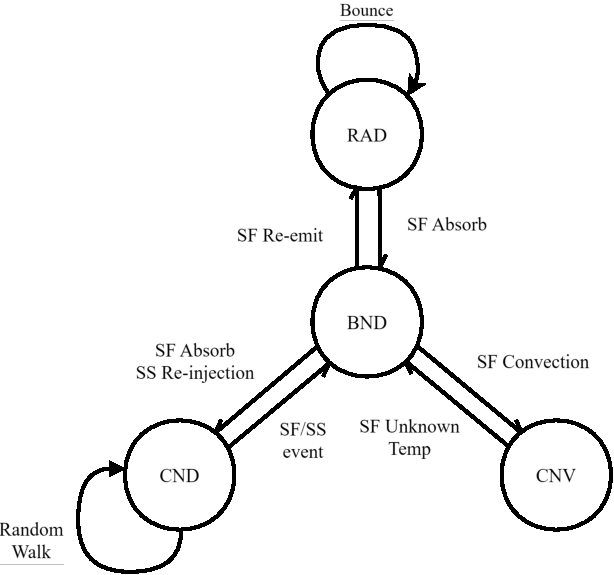
\includegraphics[width=0.6\textwidth]{Figures/Coupled_Path_Meta_SM/CPML.pdf}
  \bicaption{耦合路径的四模态转换关系图}{Module-level transition graph of coupled heat transport path}
  \label{fig:coupled_path_meta}

  \small
  四个节点分别对应辐射（RAD）、界面（BND）、传导（CND）、对流（CNV）模块，
  有向边标注触发模态转换的物理事件。路径在同一路径空间中按概率在各模态间切换，
  第三章将进一步展开每个模块内部的有限状态机设计。
\end{figure}

框架中的路径由三类路径段按物理规律拼接而成：
\begin{itemize}
    \item 辐射段（RAD）：光子在透明介质中沿直线传播，方向不变、强度不衰减（漫射灰体简化下），路径步进由几何相交查询驱动，直至命中固体表面触发界面事件（BND）。
    \item 传导段（CND）：热量在固体内通过布朗随机游走（Brownian motion）传输。更一般地，考虑含体积热源的稳态传导方程（Poisson 方程）$k\nabla^2\theta + q = 0$ 在域 $\Omega$ 上的 Dirichlet 问题 $\theta|_{\partial\Omega} = g$，Feynman-Kac 公式\cite{kacRandomWalkTheory1947}将其解表示为布朗路径的期望：
    \begin{equation}
        \theta(\mathbf{x}) = E_{\mathbf{x}}\!\left[g(B_\tau) + \int_0^\tau \frac{q(B_s)}{2k}\,\mathrm{d}s\right]
        \label{eq:feynman_kac}
    \end{equation}
    其中 $B_t$ 为从 $\mathbf{x}$ 出发的标准布朗运动（生成元 $\frac{1}{2}\nabla^2$），$\tau = \inf\{t > 0 : B_t \in \partial\Omega\}$ 为首次到达边界的停止时间。右端第一项 $g(B_\tau)$ 为路径终止于边界时读取的边界温度；第二项为路径沿途累加的体积热源贡献——每一步随机游走处的功率密度 $q$ 通过 Green 函数系数转化为温度增量。当 $q=0$ 时退化为经典 Kac 公式 $\theta(\mathbf{x}) = E[g(B_\tau)]$\cite{treganCouplingRadiativeConductive2023}。类似地，界面处指定的表面热流密度（Neumann 条件）也在路径经过时以对应系数累加为温度贡献。Feynman-Kac 公式使传导问题的蒙特卡洛求解与辐射路径追踪在形式上统一：两者都沿随机路径追踪，沿途累加源项，终止于已知边界。该公式的成立依赖传导方程的线性性——传导方程的 Green 函数恰好是布朗运动的转移概率密度。这一线性性要求是 2.1.4 中 Constraint 5（$h_R$ 线性化）的数学根源：辐射项的 $\sigma T^4$ 非线性在线性化后才能纳入随机游走框架。上述公式是稳态特例；对于瞬态传导方程 $\partial\theta_S / \partial t = \alpha \nabla^2 \theta_S$，Bati 等人\cite{batiCouplingConductionConvection2023}将有限差分空间离散后的扩散方程改写为指数分布的时间回退（backward time jump）形式：每一步 $\delta$-球面游走采样指数分布的回退时长 $T_{b,\text{cond}} \sim \mathrm{Exp}(\tau_\text{cond})$（均值 $\tau_\text{cond} = \rho c_p \tilde{\delta}^2 / (6k)$，即 $\delta$-球面尺度上的传导弛豫时间），将路径时间从观测时刻 $t$ 向初始时刻 $t_I$ 回退。若 $t - T_{b,\text{cond}} \leq t_I$，路径终止并返回初始温度场 $\theta_S(\mathbf{x}, t_I)$；否则继续游走。辐射在透明介质中以光速传播，渡越时间相对于传导弛豫时间可忽略，因此辐射段（RAD）不涉及时间回退。
    \item 对流段（CNV）：路径到达施加对流边界条件的固-流界面时，以 $P_\text{conv}$ 概率选择对流分支。该段同样携带时间回退机制：采样指数分布的回退时长 $T_{b,\text{conv}} \sim \mathrm{Exp}(\tau_\text{conv})$（均值 $\tau_\text{conv} = \rho c V / (h\mathcal{S})$，为流体腔的对流弛豫时间），若回退至 $t \leq t_I$ 则返回初始流体温度 $\theta_F(t_I)$；否则在流体腔的固-流界面上按对流系数 $h$ 加权采样一个位置，取该处固体侧温度作为流体温度的无偏估计，路径随后从该采样位置继续进入下一轮界面分叉。
\end{itemize}

三类路径段在固-流界面处（BND 过程）以随机方式发生模态转换：路径按界面物理参数决定的概率随机选择进入 CND（传导游走）、CNV（对流采样）或 RAD（辐射再发射）模块（详见下文界面耦合方程）。Bati 等人框架的一个显著特性是路径权重恒为 $W = 1$（单位权重）\cite{batiCouplingConductionConvection2023}：在每个事件点，路径以物理导出的精确概率选择分支——三模态概率来自能量守恒、俄罗斯轮盘赌吸收率 $\varepsilon$ 精确等于物理吸收率、余弦加权方向采样与辐射通量核 $\cos\theta / \pi$ 精确匹配——采样概率与被积函数权重精确相消，全程无需额外的权重修正因子。

在该框架下，路径终止于且仅终止于以下两类条件之一：(1) 路径到达温度已知的空间位置（imposed temperature），包括 Dirichlet 恒温边界和辐射路径逃逸至场景外部时读取的环境温度 $\theta_\text{env}$；(2) 传导段或对流段的时间回退累计达到初始时刻 $t_I$，路径读取初始温度场 $\theta_S(\mathbf{x}, t_I)$ 或初始流体温度 $\theta_F(t_I)$。第 (2) 类终止条件反映了传导与对流过程的瞬态弛豫特性：路径的时间坐标从观测时刻向过去回退，每经历一步传导游走或对流采样都消耗一段随机时长（指数分布，均值分别为 $\tau_\text{cond}$ 和 $\tau_\text{conv}$），当累计回退超过 $t - t_I$ 时路径即终止于初始条件。辐射段不回退时间（光速渡越可忽略），因此辐射不产生此类终止。对于稳态问题（$t - t_I \to \infty$），所有路径最终都终止于条件 (1)。

对任意空间点 $\mathbf{x}$ 在观测时刻 $t$ 的温度，从 $\mathbf{x}$ 出发独立发射 $N$ 条路径，每条路径经历若干次模态转换后终止于上述条件之一，记第 $i$ 条路径的终止温度为 $\theta_\text{term}^{(i)}$。由于单位权重特性，$\theta_\text{term}^{(i)}$ 本身即为 $\theta(\mathbf{x}, t)$ 的无偏估计，$N$ 条路径的估计量取算术均值：
\begin{equation}
    \hat{\theta}(\mathbf{x}) = \frac{1}{N}\sum_{i=1}^{N} \theta_\text{term}^{(i)}
    \label{eq:estimator}
\end{equation}
其中 $\hat{\theta}(\mathbf{x})$ 为点 $\mathbf{x}$ 处温度的蒙特卡洛估计值，$N$ 为独立采样路径数，$\theta_\text{term}^{(i)}$ 为第 $i$ 条路径的返回值——包含路径终止于已知边界时读取的温度（Dirichlet 边界温度、环境温度或初始温度场），以及路径沿途经过的体积热源和表面热流密度对温度的累加贡献（式\,\ref{eq:feynman_kac} 中的积分项）。该公式是等权算术均值而非加权和——这正是单位权重特性的直接体现：若路径携带非单位权重 $W^{(i)} \neq 1$，则估计量应为 $\hat{\theta} = \sum W^{(i)}\theta_\text{term}^{(i)} / \sum W^{(i)}$。估计量的物理含义取决于起始模态：从探测器像素出发的路径估计辐射温度（经 $L = \sigma\theta^4/\pi$ 变换为辐射亮度），从固体内部点出发的路径估计该点在时刻 $t$ 的温度。

\textbf{固-流界面（S-F）耦合}。在固-流界面处，固体侧传导热通量等于流体侧对流通量与辐射通量之和。Bati 等人通过有限差分线性化将此能量守恒条件改写为概率期望形式，使界面温度可表示为三种传输模态贡献的概率加权和\cite{batiCouplingConductionConvection2023}：
\begin{equation}
  \theta_S(\mathbf{x}) = P_\text{cond}\,\theta_S(\mathbf{x}-\delta\hat{n})
  + P_\text{conv}\,\theta_F
  + P_\text{rad}\int_{2\pi}\theta_R\,\frac{\boldsymbol{\omega}\cdot\hat{n}}{\pi}\,\mathrm{d}\boldsymbol{\omega}
  \label{eq:interface_temp}
\end{equation}
其中 $\theta_S(\mathbf{x}-\delta\hat{n})$ 为沿法线向固体内部偏移 $\delta$ 处的温度（传导贡献），$\theta_F$ 为对流流体温度，$\theta_R$ 为辐射温度。三个概率由界面物理参数决定：
\begin{equation}
  P_\text{cond} = \frac{k/\delta}{k/\delta + h + h_R}, \quad
  P_\text{conv} = \frac{h}{k/\delta + h + h_R}, \quad
  P_\text{rad} = \frac{h_R}{k/\delta + h + h_R}
  \label{eq:interface_probs}
\end{equation}
其中 $k$ 为固体导热系数，$h$ 为对流换热系数，$h_R = 4\sigma\varepsilon\theta_\text{ref}^3$ 为辐射线性化等效换热系数。辐射项中的 $T^4$ 非线性使联合边界条件无法直接改写为线性概率形式。Bati 等人\cite{batiCouplingConductionConvection2023}采用线性化处理：在参考温度 $\theta_\text{ref}$ 附近对 $\sigma T^4$ 截取一阶 Taylor 展开，由此定义 $h_R = 4\sigma\varepsilon\theta_\text{ref}^3$，将辐射通量近似为与 $T$ 的线性关系，使三模态概率可在给定 $\theta_\text{ref}$ 下预先计算且恰好满足 $P_\text{cond} + P_\text{conv} + P_\text{rad} = 1$。$\theta_\text{ref}$ 的准确度直接影响线性化误差——当实际温度与 $\theta_\text{ref}$ 偏差较大时，$h_R$ 偏离真值，导致概率失准。为此，Bati 等人在论文展望部分引入 Null-collision 接受/拒绝机制（2.2.3）：以 $h_R$ 上界计算概率，采样后根据实际温度决定接受或拒绝，保证估计量无偏。路径在界面处按上述概率随机选择进入 CND（传导游走）、CNV（对流采样）或 RAD（辐射再发射）模块，实现了三种传热模态在同一路径空间中的概率耦合。

当路径以 $P_\text{conv}$ 概率选择对流分支时，需估计流体温度 $\theta_F$。该框架将 $\theta_F$ 表示为流体腔封闭面上固-流界面温度的加权期望\cite{batiCouplingConductionConvection2023}：
\begin{equation}
  \theta_F = E\bigl[\theta_S(X_S)\bigr], \quad X_S \sim p_h(\mathbf{x}) \propto h(\mathbf{x})
  \label{eq:fluid_temp}
\end{equation}
即在流体腔的固-流界面上按对流系数 $h$ 分布采样一个位置 $X_S$，取该处固体侧温度作为 $\theta_F$ 的无偏估计。路径随后继续从 $X_S$ 处的界面进入下一轮耦合分叉。

\textbf{固-固界面（S-S）耦合}。当传导游走路径到达两个相邻固体的接触面时，物理方程为传导通量连续条件\cite{batiCouplingConductionConvection2023}：
\begin{equation}
  \theta_S(\mathbf{x}) = P_{\text{cond},1}\,\theta_S(\mathbf{x}-\delta_1\hat{n})
  + P_{\text{cond},2}\,\theta_S(\mathbf{x}+\delta_2\hat{n})
  \label{eq:ss_interface}
\end{equation}
其中 $P_{\text{cond},1} = (k_1/\delta_1)/(k_1/\delta_1 + k_2/\delta_2)$，$P_{\text{cond},2} = 1 - P_{\text{cond},1}$。路径以此概率选择注入固体 1 或固体 2 侧的 $\delta$ 偏移处，继续传导游走。固-固界面不涉及辐射和对流模态，分叉结构仅为二元导热概率选择。


\subsection{递归路径追踪求解器}
%% 写作思路：
%%   - 以 Bati Appendix B 的 4 个互递归算法为线索，取代代码结构线索。
%%   - 4 个子例程（BND/RAD/CND/CNV），每个返回温度值。
%%   - 尾递归、无权重累乘、终止于 Dirichlet 边界或环境温度。
%% [引用需求] \cite{batiCouplingConductionConvection2023}

基于上述耦合路径追踪框架，Bati 等人\cite{batiCouplingConductionConvection2023}给出了由四个互递归子例程构成的递归求解器（附录 B, Algorithms 1--4），每个子例程对应一种传热模态或界面分发过程，返回值均为温度。对任意探测点 $\mathbf{x}$，温度估计量由 $N$ 条独立路径的返回值取均值得到：$\hat{\theta}(\mathbf{x}) = \frac{1}{N}\sum_{i=1}^{N}\theta_\text{term}^{(i)}$。

四个子例程的物理含义与递归关系如下。界面分发（BND，算法\,\ref{alg:bnd}）是耦合的核心枢纽：路径到达固体界面时，首先识别界面类型（固-流或固-固），然后按物理概率将路径分发至相应的传热模态。辐射子路径（RAD，算法\,\ref{alg:rad}）沿当前方向执行光线追踪，循环处理反射/吸收事件直至被表面吸收或逃逸至环境。传导子路径（CND，算法\,\ref{alg:cnd}）在固体内执行 $\delta$-球面随机游走，每步沿随机方向前进并回退时间，直至到达初始时刻或固体边界。对流子路径（CNV，算法\,\ref{alg:cnv}）采样对流时间常数并回退时间，到达初始时刻返回流体温度，否则在固-流界面上按对流系数加权采样位置后重新进入界面分发。

\begin{algorithm}
\caption{界面分发子例程（BND）}
\label{alg:bnd}
\begin{algorithmic}[1]
\REQUIRE 界面位置 $\mathbf{x}$，当前时间 $t$
\ENSURE 温度 $\theta$
\IF{$\mathbf{x}$ 在固-固界面（S-S）}
  \STATE 计算 $P_{\text{cond},1},\,P_{\text{cond},2}$（基于两侧 $k/\delta$，式\,\eqref{eq:ss_interface}）
  \STATE 随机选择侧 $i$ $\rightarrow$ \textbf{return} \textsc{ConductiveSubpath}($\mathbf{x} + \delta_i\hat{n}_i,\,t$)
\ELSIF{$\mathbf{x}$ 在固-流界面（S-F）}
  \STATE 计算 $P_\text{conv},\,P_\text{cond},\,P_\text{rad}$（式\,\eqref{eq:interface_probs}）
  \STATE $r \leftarrow \mathrm{uniform}[0,1)$
  \IF{$r < P_\text{conv}$}
    \STATE \textbf{return} \textsc{ConvectiveSubpath}($t$)
  \ELSIF{$r < P_\text{conv} + P_\text{cond}$}
    \STATE \textbf{return} \textsc{ConductiveSubpath}($\mathbf{x} - \delta\hat{n},\,t$)
  \ELSE
    \STATE $\hat{\boldsymbol{\omega}} \leftarrow$ 余弦加权半球采样
    \STATE \textbf{return} \textsc{RadiativeSubpath}($\mathbf{x},\,\hat{\boldsymbol{\omega}}$)
  \ENDIF
\ENDIF
\end{algorithmic}
\end{algorithm}

\begin{algorithm}
\caption{辐射子路径（RAD）}
\label{alg:rad}
\begin{algorithmic}[1]
\REQUIRE 位置 $\mathbf{x}$，方向 $\hat{\boldsymbol{\omega}}$
\ENSURE 温度 $\theta$
\LOOP
  \STATE $s \leftarrow$ 沿 $\hat{\boldsymbol{\omega}}$ 光线追踪求最近交点
  \IF{$s = \infty$（未命中）}
    \STATE \textbf{return} $\theta_\mathrm{env}$ \COMMENT{环境温度}
  \ENDIF
  \STATE $\mathbf{x} \leftarrow \mathbf{x} + s\hat{\boldsymbol{\omega}}$
  \IF{$\mathrm{uniform}[0,1) < \varepsilon(\mathbf{x})$}
    \STATE \textbf{return} \textsc{BoundaryDispatch}($\mathbf{x},\,t$) \COMMENT{吸收 $\rightarrow$ 界面分发}
  \ELSE
    \STATE $\hat{\boldsymbol{\omega}} \leftarrow$ 按表面 BRDF 采样新方向 \COMMENT{反射 $\rightarrow$ 继续循环}
  \ENDIF
\ENDLOOP
\end{algorithmic}
\end{algorithm}

\begin{algorithm}
\caption{传导子路径（CND）}
\label{alg:cnd}
\begin{algorithmic}[1]
\REQUIRE 位置 $\mathbf{x}$，时间 $t$
\ENSURE 温度 $\theta$
\LOOP
  \STATE $\hat{\boldsymbol{\omega}} \leftarrow$ 各向同性方向采样
  \STATE $\tilde{\delta} \leftarrow \min(\delta,\,\text{沿}\pm\hat{\boldsymbol{\omega}}\text{到最近边界距离})$
  \STATE $\Delta t \leftarrow$ 采样指数分布（均值 $\rho c_p \tilde{\delta}^2 / (6k)$）
  \STATE $t \leftarrow t - \Delta t$ \COMMENT{时间回退}
  \IF{$t \leq t_I$}
    \STATE \textbf{return} $\theta_S(\mathbf{x},\,t_I)$ \COMMENT{到达初始时刻}
  \ENDIF
  \STATE $\mathbf{x} \leftarrow \mathbf{x} + \tilde{\delta}\hat{\boldsymbol{\omega}}$
  \IF{$\mathbf{x}$ 在边界上}
    \STATE \textbf{return} \textsc{BoundaryDispatch}($\mathbf{x},\,t$) \COMMENT{到达界面 $\rightarrow$ 分发}
  \ENDIF
\ENDLOOP
\end{algorithmic}
\end{algorithm}

\begin{algorithm}
\caption{对流子路径（CNV）}
\label{alg:cnv}
\begin{algorithmic}[1]
\REQUIRE 时间 $t$
\ENSURE 温度 $\theta$
\STATE $\Delta t \leftarrow$ 采样指数分布（均值 $\tau_\text{conv}$）
\STATE $t \leftarrow t - \Delta t$ \COMMENT{时间回退}
\IF{$t \leq t_I$}
  \STATE \textbf{return} $\theta_F(t_I)$ \COMMENT{到达初始时刻 $\rightarrow$ 流体温度}
\ENDIF
\STATE $\mathbf{x}_S \leftarrow$ 在固-流界面上按 $h(\mathbf{x})$ 加权采样位置
\STATE \textbf{return} \textsc{BoundaryDispatch}($\mathbf{x}_S,\,t$) \COMMENT{采样位置 $\rightarrow$ 界面分发}
\end{algorithmic}
\end{algorithm}

上述四个子例程构成互递归调用图：BND 根据界面类型和物理概率选择模态分支，各模态子例程在路径到达新界面时回调 BND，形成递归展开。路径展开以深度优先方式进行，每次递归调用返回温度值，不涉及权重累乘——单位权重特性（\ref{sec:coupled_framework}）保证每次模态分叉的采样概率与物理贡献精确相消。路径终止于两种条件之一：(1) 到达已知温度的 Dirichlet 边界或环境温度；(2) 时间回退至初始时刻 $t_I$。

此递归结构在正确性上完整复现了 \ref{sec:coupled_framework} 的耦合路径追踪框架理论。然而，其将路径状态隐式绑定于函数调用栈的实现特性——四个子例程的互递归展开导致路径的全部中间状态分散于多层栈帧中，既不可序列化也不可中断恢复——构成了面向并行化改造时的深层结构性障碍，下一小节将从四个递推角度展开分析。

\subsection{递归求解框架的局限性分析}
\label{sec:dfs_limitations}

2.2.5 的递归求解器通过同步阻塞的几何查询调用驱动路径状态机前进：每次查询提交后函数原地等待结果返回，然后依据结果执行后续物理计算。对该求解器控制流的完整分析表明，一条路径从发射到终止典型需经历 50--200 次同步几何查询，最坏情况可达数千次，且每次均以宽度为 1 的串行方式执行。虽然不同像素间的路径在统计层面完全独立，但递归求解器在架构层面将这种并行潜力完全放弃。以下从四个相互递推的角度分析其结构性障碍，四者均源于同一根因：路径状态与执行控制流的隐式耦合。

\subsubsection{障碍 A：调度粒度过大}

递归求解器将路径完整求解过程封装为一次连续的函数调用链，涵盖 RAD、BND、CND、CNV 全部物理逻辑。若将该调用链直接映射到单一 GPU kernel（即 MegaKernel 方案），则 kernel 体积极大，寄存器需求量极高，且递归深度受 GPU 栈空间严格限制——GPU 单 SM 的 warp 占用率远低于理论峰值。即便忽略栈深度限制，同一 warp 内各路径所处物理阶段不同（部分执行 RAD 弹射，部分处于 CND 游走，部分进入 BND 概率分叉），指令路径严重分叉，SIMT 执行效率大幅下降。

\subsubsection{障碍 B：路径状态不可持久化}

更深层的障碍在于递归求解器的状态保存方式。路径的全部中间状态（位置、方向、权重、路径深度、随机数状态等）分散在多层调用栈帧的局部变量中，是程序控制流的副产物而非独立数据对象。这些信息无法在函数调用途中以完整快照形式导出：函数若不等待查询结果便无法正常返回，而强行返回则栈帧释放、中间状态不可恢复地丢失。因此路径执行不具有中断、挂起与恢复的能力。

\subsubsection{障碍 C：几何查询请求无法批量积累}

批量化要求在同一时刻积累多条路径的查询请求后统一提交。该要求以两个条件为前提：(1) 多条路径能同时推进到各自的查询节点；(2) 存在统一的调度视角收集这些请求。递归求解器的同步阻塞结构使两个条件均不成立——第一条路径的查询调用占用控制流直至结果返回，其他路径无法推进；即使多线程化，各线程各自独立阻塞，系统不存在能观察全部等待路径的全局调度节点。几何查询提交宽度恒为 1，无法触及 SIMD packet 批量接口，更无法将请求卸载至 GPU 硬件光追管线。

\subsubsection{障碍 D：复合物理分支无法拆分调度}

路径在 BND 界面事件中产生复合物理分支：以概率 $\varepsilon$ 吸收转入传导/对流，以 $1-\varepsilon$ 漫反射继续辐射传播；null-collision 循环内还可能递归生成子路径树以评估辐射贡献。这些分支以嵌套函数调用形式展开，分叉发生在运行时且依赖查询结果，不同路径的分支选择完全异步——若将不同分支处的路径混合调度，无法统一选定推进方向，形成闭环依赖。

\subsubsection{局限性总结}

四大障碍层层递推：路径状态绑定于调用栈（障碍 B）导致不可挂起，使查询请求无法跨路径积累（障碍 C）；调度粒度锁定在完整路径生命周期（障碍 A），叠加物理分支无法拆分（障碍 D），使递归求解架构下任何批量化策略均不可行。要实现批量化，必须将路径状态从调用栈中显式提取为独立的可序列化数据结构，将状态推进与几何查询执行解耦为两个独立阶段——这正是 2.3 Wavefront 执行模型的设计出发点，也是第三章 Wavefront 求解器实现的直接依据。

\section{Wavefront 执行模型}
%% [篇幅需求] 约1000字，重在阐明批量化障碍与解耦范式，无需深入第三章的实现细节。
%% [写作总思路]
%%   从 DFS 固有的同步耦合结构出发（2.3.1），引出 Wavefront 解耦范式（2.3.2），
%%   最后分析对耦合热输运的适用性并如实交代解耦引入的 Cache 代价（2.3.3）。
%%   不以 GPU Warp 发散为主逻辑链，而以"DFS 1-宽度同步结构无法积累批量查询"为核心动机。

\subsection{从递归求解框架的障碍到批量化需求}
%% 简要衔接 2.2.6 与 Wavefront 范式

2.2.6 的四大障碍分析揭示了递归求解架构无法实现批量几何查询的根本结构性原因：路径状态与执行控制流的隐式耦合。其中，障碍 B（路径状态不可持久化）和障碍 C（查询请求无法批量积累）指向最直接的解法方向——将状态推进与查询执行从同一控制流中解耦为两个独立阶段。这正是 Wavefront 执行范式的核心思想。

\subsection{Wavefront范式：解耦状态推进与查询执行}
%% 写作思路：
%%   - 核心思想（硬件无关）：路径维护持久化状态结构体，CPU 推进路径状态机；
%%     当路径抵达需要几何查询的节点时，将请求写入挂起队列（pending queue），
%%     路径进入 PENDING 状态挂起；CPU 继续推进其他路径；
%%     积累完毕后统一提交给几何查询后端；结果返回后路径从 PENDING 恢复继续推进。
%%   - Laine et al. 2013 起源（一句带过）：原始动机是解决 GPU Megakernel 的 Warp 发散
%%     和寄存器压力问题，但解耦结构的价值独立于具体硬件。
%%   - 本文三类 PENDING：RT（射线最近命中）、ENC（封闭腔体归属查询）、
%%     CP（最近面投影），三类由耦合热输运物理过程决定；Wavefront 使其自然积累
%%     为批量请求，后端如何高效执行是独立设计问题（第四章）。
%% [图表需求] Wavefront 双阶段循环示意（CPU 推进阶段 → pending queue → GPU 执行阶段 → 恢复）
%% [引用需求] \cite{laineMegakernelsConsideredHarmful2013}

Wavefront 范式通过引入持久化路径状态与挂起队列机制，在架构层面将状态推进与查询执行分离为两个独立的执行阶段。每条路径拥有一个长期驻留于内存的状态结构体，记录其当前位置、方向、累积权重、命中信息及物理状态标识。CPU 推进阶段遍历所有路径，逐条将其在状态机中向前推进；当某条路径到达需要几何查询的节点时，CPU 将该查询请求写入对应的挂起队列（pending queue），路径进入 PENDING 状态等待，CPU 立即继续处理下一条路径，而不阻塞等待。待本轮推进完成，所有进入 PENDING 的路径已自然积累为一批同类查询请求，统一提交至几何查询后端执行。后端执行阶段完成批量查询后，将结果写回各路径的状态结构体，路径从 PENDING 状态恢复，等待下一轮 CPU 推进阶段继续向前。上述两阶段交替循环，直至所有路径终止采样。

这一范式最早由 Laine 等人在 GPU 路径追踪场景中以"Wavefront"之名提出，彼时的原始动机是解决 Megakernel 架构下因路径状态异质而导致的 Warp 发散与寄存器压力问题。然而，解耦结构的核心价值——将状态推进与查询执行分离，使批量查询自然涌现——独立于 GPU 硬件存在：在 GPU 上，挂起路径对应 kernel 间的全局显存队列；在 CPU 多线程实现中，挂起路径则对应线程池共享的内存数组，同样可获得批量积累的效果。

在耦合热输运求解中，几何查询并非单一类型，而是按用途分为三类，各自对应不同的查询语义与 GPU 实现管线：RT 查询（ray tracing，沿路径方向找到第一个几何交点，驱动所有涉及直接射线求交的物理过程）、ENC 查询（enclosure，给定空间点判断其所属封闭腔体，用于 BND 界面事件中的腔体归属判断）、CP 查询（closest point，给定空间点求场景表面最近点，仅用于传导段 CND 中 Walk-on-Spheres 游走路径的步长计算）。路径推进至需要上述任一查询时即进入对应类型的 PENDING 状态，三类挂起队列在每轮推进后各自积累为一组同类批量请求统一提交。三类查询的语义与分类由耦合热输运的物理过程决定，而非由特定后端驱动；Wavefront 框架使这些请求自然地以批量形式呈现给查询后端，后端如何高效处理这些批量请求则是独立于 Wavefront 范式之外的工程设计问题。

\subsection{适用性分析与解耦引入的 Cache 代价}
%% 写作思路：
%%   - 适用性：四状态路径与渲染路径同构，CPU 线性遍历路径数组自然积累三类 PENDING，
%%     无需按状态排序分桶（排序引入数据重排开销，路径数有限时收益不明显）。
%%   - Cache 代价：DFS 对照组仅维护单条路径的栈上状态（L1 完全覆盖）；
%%     Wavefront 需同时维护 N 条路径的持久化结构体（工作集远超缓存容量），
%%     遍历时对每条路径的随机访问几乎均为 cache miss，是本实现头号性能瓶颈。
%%   - 此代价与架构绑定，是实现解耦的必要代价；优化方向（SoA 布局等）留给第三章。
%% [引用需求] \cite{laineMegakernelsConsideredHarmful2013}

耦合热输运路径在 RAD/BND/CND/CNV 四类状态间按物理规律切换，与图形渲染路径的状态机结构高度同构，Wavefront 范式对本问题天然适用。在具体实现中，CPU 推进阶段只需按顺序线性遍历路径数组，逐条将各路径推进至下一个 PENDING 节点，无需预先对路径按状态排序分桶——分桶操作涉及额外的数据重排开销，且在路径总数有限的工程场景中收益不明显；三类 PENDING 挂起队列中的查询请求在遍历过程中自然积累，作为本轮推进的副产品直接送达后端。

然而，解耦带来的批量查询能力是以一项新的 Cache 代价为前提的，该代价在递归求解器对照组中完全不存在。在递归求解器框架中，同一时刻只有一条路径处于活跃状态，其全部状态数据（位置、方向、权重、命中信息等）驻留于 CPU 调用栈上，体量极小，可完全驻留于 L1 缓存，访问延迟可忽略不计。而 Wavefront 实现需要同时将 $N$ 条路径的状态结构体长期保存于主存——$N$ 越大，积累的批量查询规模越大，查询后端可从中获取更高的并行执行效率；但 $N$ 个结构体构成的内存工作集随 $N$ 的增大迅速超出 CPU 末级缓存（LLC）的容量。CPU 推进阶段线性遍历路径数组时，对每条路径状态结构体的访问在缓存中几乎均无命中，频繁触发 cache miss 与主存访问，产生显著的访问延迟。这一 Cache 压力是本实现相对对照组引入的独有性能瓶颈，也是驱动第三章中状态结构体布局优化（结构体数组 AoS 与数组结构体 SoA 的权衡）等设计决策的直接原因。

综上，Wavefront 范式的核心贡献是将状态推进与查询执行解耦，使大批量几何查询从架构层面成为可能；其代价是持久化路径状态数组带来的 Cache 压力。正确认识这一权衡，是理解本文混合架构设计选择和第三章性能分析的基础。

\section{光线追踪与几何查询加速技术}
%% [篇幅需求] 约2000字，从算法原理到工程实现，为第四章 OptiX 后端的设计决策提供理论依据。
%% [写作总思路]
%%   先讲光线-几何求交的基础算法（2.4.1），再介绍使求交加速几个数量级的 BVH 加速结构（2.4.2），
%%   然后分别介绍 CPU（2.4.3）和 GPU（2.4.4）两条工程实现路线，
%%   最后扩展到本文实际需要的三类几何查询（2.4.5），为第四章的后端管线设计直接铺垫。

\subsection{光线-几何求交算法}
%% [写作思路（已修订）]
%%   - 问题定义：光线参数方程，求最近交点 $(t^*, u^*, v^*)$。
%%   - Möller-Trumbore（MT）算法：Cramer 法则直接求解，简洁高效，是概念参考实现。
%%     但 MT 不满足水密性：共享棱边/顶点处两相邻三角形独立计算，浮点舍入可能导致
%%     双重漏判（穿透缝隙）或双重命中（虚假散射）。
%%   - 为什么需要水密性：封闭网格表示真实物理固体边界；穿透缝隙令蒙特卡洛粒子泄入
%%     错误腔体，破坏腔体归属和权重贡献；低仰角红外成像场景（掠角观测）对此最为敏感。
%%   - WBW（Wald-Benthin-Woop）水密算法：将求交变换到射线对齐坐标系，以棱函数的
%%     符号一致性判别消除共享棱/顶点歧义，保证相邻三角形各自对共享边界唯一所有权。
%%   - WBW 是工业实施标准：Embree 默认求交内核（配合 SIMD 批量）；
%%     NVIDIA RT Core 固定功能求交电路的硬件设计基础。
%% [公式需求] 光线参数方程、MT Cramer 解、WBW 棱函数
%% [引用需求] \cite{MollerTrumbore1997,WaldBenthinWoop2013}

光线追踪的基本操作是给定一条射线，在三角形网格场景中快速求出最近交点。射线以参数方程定义：
\begin{equation}
    \mathbf{r}(t) = \mathbf{o} + t\hat{\mathbf{d}}, \quad t \in [t_{\min},\, t_{\max}]
    \label{eq:ray}
\end{equation}
其中 $\mathbf{o}$ 为原点，$\hat{\mathbf{d}}$ 为归一化方向，$t_{\min} > 0$ 用于排除起点处的自相交，$t_{\max}$ 为远截面截断。对顶点坐标为 $\mathbf{p}_0, \mathbf{p}_1, \mathbf{p}_2$ 的三角形，命中条件等价于求解线性方程组：
\begin{equation}
    \mathbf{o} + t\hat{\mathbf{d}}
    = (1 - u - v)\,\mathbf{p}_0 + u\,\mathbf{p}_1 + v\,\mathbf{p}_2,
    \quad u \geq 0,\; v \geq 0,\; u + v \leq 1
    \label{eq:mt_system}
\end{equation}
令 $\mathbf{e}_1 = \mathbf{p}_1 - \mathbf{p}_0$，$\mathbf{e}_2 = \mathbf{p}_2 - \mathbf{p}_0$，$\mathbf{s} = \mathbf{o} - \mathbf{p}_0$，Cramer 法则直接给出 Möller-Trumbore（MT）算法：
\begin{equation}
\begin{pmatrix} t \\ u \\ v \end{pmatrix}
= \frac{1}{(\hat{\mathbf{d}} \times \mathbf{e}_2) \cdot \mathbf{e}_1}
  \begin{pmatrix}
    (\mathbf{s} \times \mathbf{e}_1) \cdot \mathbf{e}_2 \\
    (\hat{\mathbf{d}} \times \mathbf{e}_2) \cdot \mathbf{s} \\
    (\mathbf{s} \times \mathbf{e}_1) \cdot \hat{\mathbf{d}}
  \end{pmatrix}
\label{eq:moller_trumbore}
\end{equation}
MT 算法结构极为简洁——仅需 1 次叉积与 3 次点积，无需预存三角形法向量，长期作为概念参考实现广泛使用。然而，MT 算法不满足水密性（watertightness）的工程要求。

射线求交算法的水密性需求源自以下数值问题：在以三角形网格表示的封闭固体中，相邻三角形共享棱边和顶点。当射线以极小入射角掠过共享棱边时，两个相邻三角形各自独立地以浮点运算计算重心坐标，判定条件 $u \geq 0,\, v \geq 0,\, u+v \leq 1$ 的数值结果均落在零附近；不同量级的中间舍入误差可引发两类相反的不一致：若两个三角形均错误地返回"不命中"，则共享棱边处产生数值裂缝，射线得以穿透封闭表面；若两个三角形均返回"命中"，则同一边界点被重复计数，产生虚假的双重散射事件。

在蒙特卡洛耦合热输运求解中，上述两类失效均直接破坏物理正确性。穿透失效使传导段布朗游走粒子越过物理边界进入错误腔体：一旦腔体归属（\texttt{enc\_id}）出错，粒子此后所读取的材质参数、发射率及对流换热系数全部来自错误腔体，对应样本的完整权重贡献均为系统性偏差而非统计噪声，无法通过增加样本量消除。双重命中失效使辐射路径在掠角方向上被提前终止或双倍统计，引入方向相关的偏差。两类误差在低仰角红外成像（掠角观测）场景中最为集中——极小入射角正是最频繁触发共享棱边临界情形的几何配置，而低仰角观测又是红外探测的重要应用场景。MT 算法对掠棱情形的判定结果完全依赖各三角形各自的浮点舍入，无法为相邻三角形之间建立任何一致性保证，不能满足物理仿真对几何边界一致性的严格要求。

为了满足水密性要求，Wald、Benthin 与 Woop 提出将求交问题变换到射线对齐坐标系（ray-aligned frame）中处理，以彻底消除共享棱边/顶点处的分类歧义\cite{woopWatertightRayTriangle2013}。算法分离线预处理与在线查询两个阶段：

\textit{预处理阶段（逐三角形，离线完成）}：对每个三角形预计算一个 $3\times 4$ 仿射变换矩阵 $M$，将世界坐标映射到以查询射线方向为 $+z$ 轴的局部坐标系——三角形在此坐标系的 $z=1$ 截面退化为标准单位三角形，三个顶点变换后的局部坐标分量记为 $(x_i, y_i, z_i)$，$i=0,1,2$。

\textit{查询阶段（逐射线，在线执行）}：以 $M$ 将光线原点变换至局部坐标后，命中判定转化为三个有符号棱函数（edge function）的符号一致性检验：
\begin{equation}
    e_0 = x_1 y_2 - x_2 y_1,\quad
    e_1 = x_2 y_0 - x_0 y_2,\quad
    e_2 = x_0 y_1 - x_1 y_0
    \label{eq:WBW_edge}
\end{equation}
当且仅当 $e_0, e_1, e_2$ 同号（均 $\geq 0$ 或均 $\leq 0$）时判定命中，命中参数为 $t = (e_0 z_0 + e_1 z_1 + e_2 z_2)/(e_0 + e_1 + e_2)$。水密性的关键在于：将 $e_i = 0$（射线恰好掠过该棱边）归入正方向一侧——即 $0$ 满足"$\geq 0$"——保证共享此棱边的相邻两三角形中恰好一个声明对边界点的所有权，另一个三角形对应的棱函数值与之互为相反符号，被排除在命中判定之外，从而在数学上彻底消除双重命中与双重漏判的可能性。

WBW 算法是现代高性能光追软件与图形硬件的实施标准。Intel Embree 将 WBW 求交内核与 SIMD 指令相结合，通过射线包（ray packet）模式同时对 4/8/16 条射线执行批量坐标变换与符号判别，在保证水密性的同时充分利用向量并行能力。NVIDIA 自 Turing 架构起引入的 RT Core 硬件固定功能单元，其内部求交电路以 WBW 坐标变换与棱函数符号一致性逻辑为核心，在晶体管层面实现了每时钟周期完成多组射线—三角形水密求交的全流水线设计。正是这一从算法到硬件的统一实施路线，确保了在任意复杂封闭网格场景中，几何表面对光线路径和随机游走粒子始终是严格不可穿透的。

\subsection{层次包围体加速结构}
%% 写作思路：
%%   - 暴力检测的复杂度：$O(N)$（$N$ 为三角形数），大规模场景（百万面片）不可接受。
%%   - BVH 的核心思想：将场景三角形组织为二叉树，每个节点包含其子树所有三角形的
%%     轴对齐包围盒（AABB）；光线先与包围盒测试，快速剔除不相交的子树，平均复杂度降至 $O(\log N)$。
%%   - 构建策略：SAH（Surface Area Heuristic）——估计划分代价 $C = c_t + \frac{A_L}{A} N_L c_i + \frac{A_R}{A} N_R c_i$，
%%     选使代价最小的分割轴和分割点；实践中用 binning 近似以控制构建时间。
%%   - 遍历算法：栈式深度优先，子节点按 $t_\text{near}$ 排序（近者先访问），
%%     及时利用当前最近距离 $t^*$ 剪枝。
%%   - 其他加速结构简述（一句话）：KD-Tree（更紧凑但构建慢）、Grid（均匀分布场景有效）。
%% [公式需求] SAH 代价函数
%% [图表需求] BVH 树结构示意图（左：场景包围盒层次；右：对应的二叉树节点）
%% [引用需求] \cite{ailaUnderstandingEfficiencyRay2009}

对场景所有三角形逐一进行光线—三角形求交的暴力算法复杂度为 $O(N)$（$N$ 为三角形总数），在包含数百万面片的实际工程场景中完全不可接受。层次包围体加速结构（Bounding Volume Hierarchy，BVH）是现代高性能光线追踪系统的基础加速数据结构，可将单次查询的期望复杂度从 $O(N)$ 压缩至 $O(\log N)$。

BVH 将场景中所有三角形递归地组织为一棵二叉树：每个内部节点存储其子树所有三角形的轴对齐包围盒（Axis-Aligned Bounding Box，AABB），叶节点存储少量三角形（通常 1～8 个）。遍历时，从根节点出发，光线先以解析公式与子节点 AABB 作快速相交测试；若光线与某 AABB 不相交，则跳过其下方所有几何体；若相交，则递归进入子节点，直至到达叶节点后对实际三角形执行精确求交。通过层次剔除，期望仅需访问 $O(\log N)$ 个节点即可完成最近交点查询。

BVH 的划分质量直接决定遍历效率，工程中普遍采用面积启发式（Surface Area Heuristic，SAH）作为划分准则。SAH 以包围盒表面积之比估计随机光线命中某子树的概率，量化每种候选划分的预期遍历代价：
\begin{equation}
    C = c_t + \frac{A_L}{A}\,N_L\,c_i + \frac{A_R}{A}\,N_R\,c_i
    \label{eq:sah}
\end{equation}
其中 $c_t$ 为包围盒测试代价，$c_i$ 为三角形求交代价，$A_L$、$A_R$ 分别为左右子节点 AABB 的表面积，$A$ 为父节点 AABB 的表面积，$N_L$、$N_R$ 为对应子节点包含的三角形数。在每个候选分割轴（$x/y/z$）上扫描所有候选分割位置，取使式\,\eqref{eq:sah} 最小的轴与位置作为最优划分；实践中以binning 近似（将候选位置离散为 32～64 个等宽桶）替代精确全局搜索，可将构建复杂度控制在 $O(N\log N)$ 以内而不显著损失划分质量。

BVH 遍历采用栈式深度优先策略：维护一个节点索引栈，每次弹出栈顶节点后对其两个子节点分别执行 AABB 测试；通过测试的子节点按 $t_\mathrm{near}$（光线进入包围盒的最小参数值）由小到大压栈，优先探索距离更近的子树。一旦在近子树中找到交点 $t^*$，即可对满足 $t_\mathrm{near} > t^*$ 的远处节点直接跳过（剪枝），大幅减少访问节点数量。除二叉 BVH 外，KD-Tree 提供更紧凑的空间划分但构建代价更高，均匀网格（Grid）在几何分布均匀场景下有效但空间利用率低；现代高性能光追库（Embree、OptiX）均以 BVH 为核心，并将其扩展为 4 叉或 8 叉宽树以配合 SIMD 指令或 RT Core 并行执行。

\begin{figure}[htbp]
  \centering
  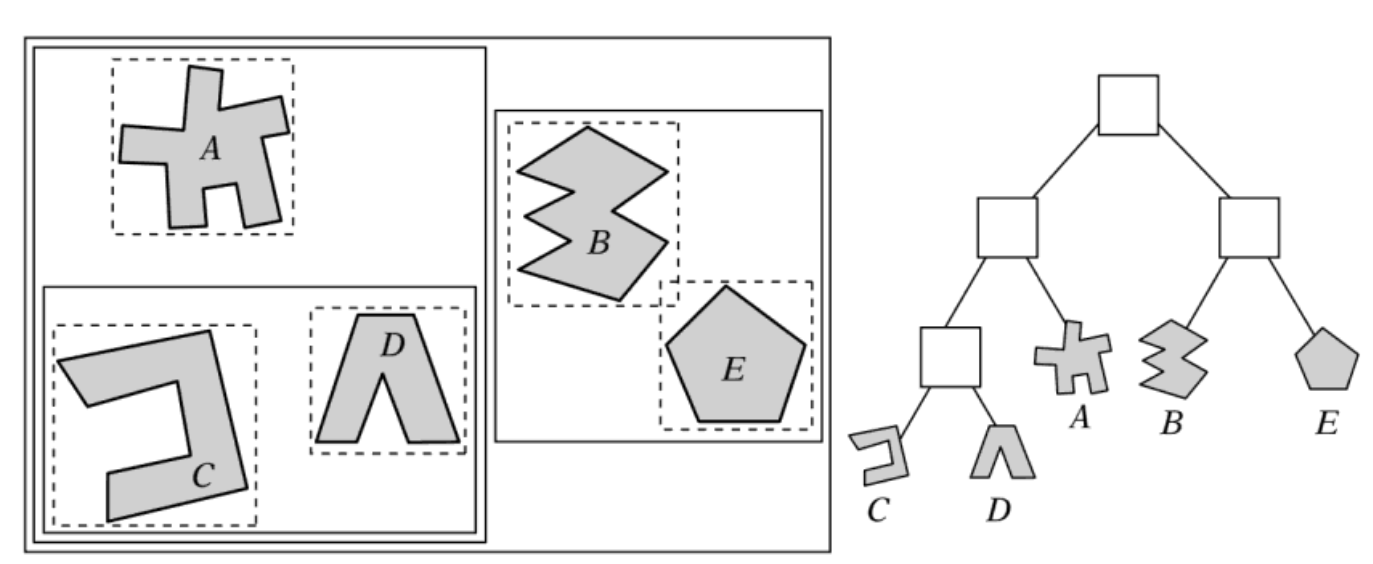
\includegraphics[width=0.85\textwidth]{Figures/BVH/BVH.png}
  \bicaption{BVH 加速结构示意图}{Schematic of BVH acceleration structure}
  \label{fig:bvh_structure}

  \small
  场景包围盒层次（左）与对应二叉树（右）。
\end{figure}

\subsection{CPU 光追加速：Intel Embree}
%% 写作思路：
%%   - Embree 定位：Intel 开发的高性能 CPU 光线追踪内核库，是本文 CPU Baseline 求解器
%%     （stardis-cpu）的几何相交后端。
%%   - 关键技术：
%%       · SIMD 并行（SSE4/AVX2/AVX-512）：同时对 4/8/16 条射线做 packet 遍历；
%%       · 多级 BVH（MBVH）：宽度为 4 或 8 的多叉 BVH，与 SIMD 寄存器宽度对齐；
%%       · 针对不同几何类型（三角形、曲线、细分曲面）的专用相交核。
%%   - 典型性能：单线程 ~$10^7$ rays/s 量级；多核线性扩展。
%%   - 本文角色：作为 Baseline 的几何后端，与第四章 GPU 后端进行性能对比。
%% [引用需求] \cite{waldEmbreeKernelFramework2014,EmbreeRayTracing}

Intel Embree 是 Intel 开发并开源的高性能 CPU 光线追踪内核库，也是本文 CPU 基准求解器的几何相交后端。Embree 针对现代 x86 处理器的 SIMD 指令集深度优化，通过射线包（ray packet）遍历模式实现单线程内的大幅并行加速：将宽度为 4、8 或 16 的多条射线打包为一个 packet，以 SSE4（128 位）、AVX2（256 位）或 AVX-512（512 位）SIMD 指令同时完成 packet 内所有射线与 BVH 节点（包围盒测试）或三角形（求交）的计算，每条向量指令处理多条射线，显著提升单位时钟周期内的浮点利用率。

与射线包遍历配套的底层加速结构为多叉 BVH（MBVH）：将二叉 BVH 扩展为 4 叉（QBVH，对应 SSE4）或 8 叉（OBHV，对应 AVX2）树，每个内部节点同时存储 4 个或 8 个子节点的 AABB 数据，恰好填满 SIMD 寄存器。包围盒测试时，一条向量指令可并行完成对全部子节点的 AABB 测试，将每个 BVH 节点的遍历代价压缩至极低。此外，Embree 针对三角形、线段曲线、细分曲面等不同几何图元类型提供了各自优化的专用求交内核，并支持用户注册自定义几何体类型的求交回调。

Embree 对外提供宽度分级的 C API：\texttt{rtcIntersect1()}（单条射线）、\texttt{rtcIntersect4/8/16()}（4/8/16 条射线 packet，分别对应 SSE4/AVX2/AVX-512）。宽接口在路径连贯、方向分布集中的渲染场景中可充分利用 SIMD 并行能力，达到接近理论峰值的吞吐量。然而，本文基准求解器在架构层面仅使用了 \texttt{rtcIntersect1()}——递归求解器为每条路径的每次状态转换各自独立发起一次同步查询，同一时刻从不存在多条路径的查询请求同时就绪，packet 接口所要求的一批方向同构射线在递归求解器中不可能被自然积累。这一约束正是 2.3.1 所描述的批量化障碍在 Embree 接口层面的直接体现：未能使用宽 packet 的原因不是 API 能力的缺失，而是上层递归求解架构决定了路径查询只能以宽度为 1 的形式提交。典型性能下，Embree 单条射线吞吐量约 $10^7$ 条/秒量级，开启 packet 模式后可进一步提升 4--8 倍；本文基准求解器受架构限制实际仅获得前者。在本文实验框架中，Embree 作为 CPU 基准后端的几何相交底层支撑，其性能将在第四章与基于 OptiX 的 GPU 批量查询后端进行系统性对比。

值得指出的是，Embree 本身是线程安全的：多个线程可安全地并发调用同一场景句柄的查询接口，无需额外加锁。本文基准求解器利用这一特性以 OpenMP 在粒子（路径）层面实现粗粒度并行——每个 OpenMP 线程独立运行一条路径的递归求解器并各自调用 \texttt{rtcIntersect1()}，线程间几乎不存在同步开销，从而在多核 CPU 上获得接近线性的加速比。本文 Wavefront 求解器同样依托 OpenMP 实现多线程并行，不同之处在于并行粒度从单条路径转变为任务队列：各 OpenMP 线程并行处理同类型挂起队列中的多个粒子状态，以批量方式驱动状态转换。两种架构均能随核心数的增加获得近线性的多核扩展能力，差异体现在对 SIMD 向量化与 GPU 批量卸载的利用程度上。

\subsection{GPU 硬件光追加速}
%% 写作思路：
%%   - RT Core 简介（Turing 架构起，NVIDIA 第一代，Ampere 为第二代）：专用固定功能单元，
%%     独立于 CUDA Core 和 Tensor Core，负责 BVH 遍历和光线-三角形求交。
%%   - 执行流程：CUDA kernel 发出 optixTrace() 调用 → 光线进入 RT Core 流水线 →
%%     BVH 遍历与求交完全在硬件中完成（对 CUDA 透明）→ 命中后触发用户可编程的 Closest-Hit
%%     / Any-Hit / Miss Shader（在 SM 上执行）。
%%   - 性能优势：RT Core 与 SM 并行工作，在高并发查询下吞吐量可达 Embree（单核）的 5~10 倍；
%%     本文实测结果见第四章。
%%   - OptiX 编程模型：NVIDIA 提供的光线追踪 API，封装 RT Core，提供 Pipeline/SBT（Shader
%%     Binding Table）机制，支持用户自定义 Intersection/Closest-Hit/Any-Hit/Miss 程序。
%% [图表需求] GPU SM 与 RT Core 协同流水线示意图（optixTrace→RT Core→Shader 执行流程）
%% [引用需求] \cite{parkerOptiXGeneralPurpose2010}

NVIDIA 自 Turing 架构（2018 年）起在 GPU 芯片中引入了专用的固定功能硬件单元 RT Core（Ray Tracing Core），Ampere 架构（2020 年）进行了第二代升级。RT Core 独立于传统的浮点 CUDA Core 和矩阵乘法 Tensor Core，专门负责两项操作：光线与 AABB 的相交测试，以及光线与三角形基于 Woop 坐标变换的精确求交。整个 BVH 遍历与三角形求交流水线在 RT Core 硬件中完成，不占用 SM 的可编程计算资源。

在 NVIDIA OptiX 框架下，GPU 光线查询的完整执行流程为：
\begin{enumerate}
    \item CUDA kernel 中调用 \texttt{optixTrace(handle, rayOrigin, rayDirection, tmin, tmax, ...)} 提交一条射线及其查询参数（SBT 偏移、Payload 寄存器等）；
    \item RT Core 从顶层加速结构（TLAS，Top-Level Acceleration Structure）向下执行 BVH 遍历，对每个叶节点中的三角形执行 Woop 坐标求交，并记录最近命中的 $t$ 值与几何属性；
    \item 遍历完成后，根据命中结果分发到对应的用户 Shader 程序，在 SM 上执行：
    \begin{itemize}
        \item \textbf{Closest-Hit Shader} --- 在最近命中时执行，处理交点信息进行路径更新;
        \item \textbf{Miss Shader} --- 在射线未命中任何几何体时执行，处理路径终止或背景采样;
        \item \textbf{Any-Hit Shader} --- 在每次潜在命中时执行（可选，用于透明度过滤）;
        \item \textbf{Intersection Shader} --- 用户自定义的自定义几何类型求交逻辑。
    \end{itemize}
\end{enumerate}
RT Core 遍历与 SM 执行异步并行：一条 Warp 提交 \texttt{optixTrace()} 后进入挂起态，SM 调度器立即切换到其他就绪 Warp 继续执行；RT Core 在后台完成遍历，结束后重新唤醒该 Warp 执行对应 Shader。这种流水线机制在大批量查询场景下使 RT Core 与 SM 的计算资源高度重叠，整体查询吞吐量远超纯软件 BVH 遍历。

OptiX 的高层接口以管线（Pipeline）和着色器绑定表（Shader Binding Table，SBT）两个概念为核心：Pipeline 定义本次查询涉及的 Shader 程序集合（CUDA PTX，由 OptiX JIT 链接）及遍历深度等配置参数；SBT 是设备端表格，每行对应一个几何实例及其绑定的 Shader 程序与参数，\texttt{optixTrace()} 通过携带的 SBT 偏移实现对不同几何体命中不同 Shader 的精确路由。正是这一灵活的 Pipeline/SBT 机制，使本文能够在保留 RT Core 硬件加速的前提下，为三类语义不同的几何查询分别构建独立管线。

\begin{figure}[htbp]
  \centering
  % 第一排：全芯片架构
  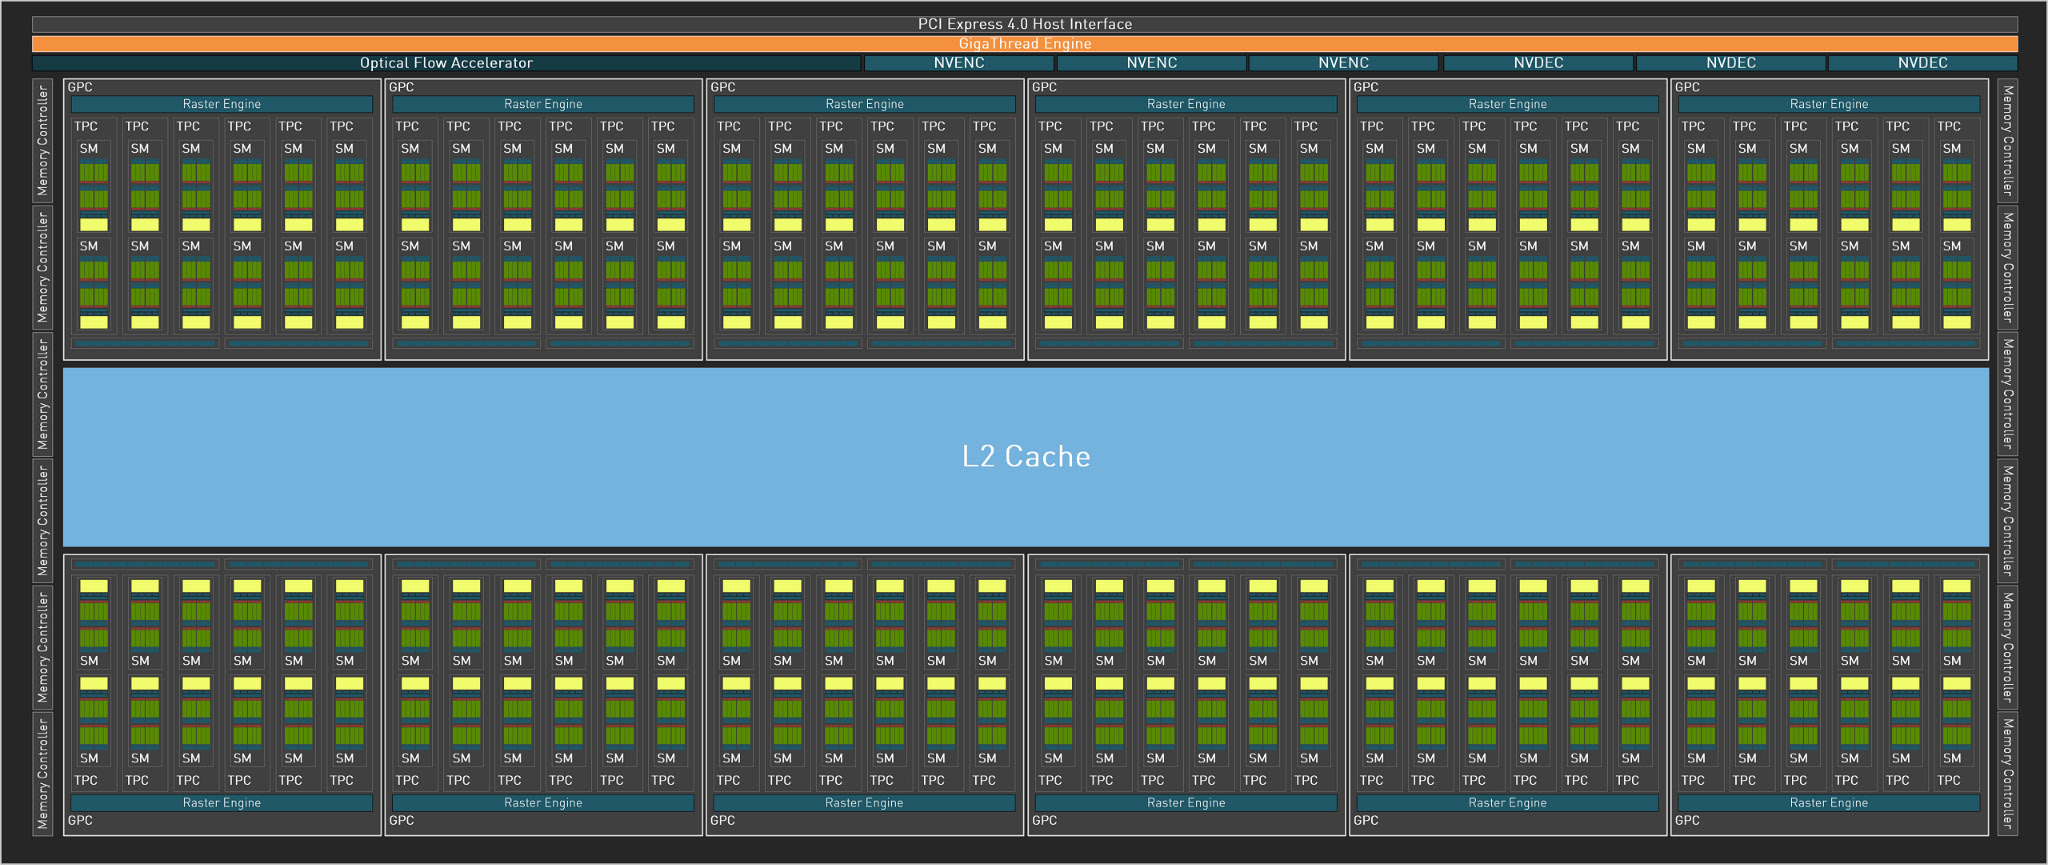
\includegraphics[width=0.95\textwidth]{Figures/GPU_Arch/AD102CoreArch.png}

  \vspace{6pt}
  % 第二排：GPC + SM
  \begin{subcaptiongroup}
  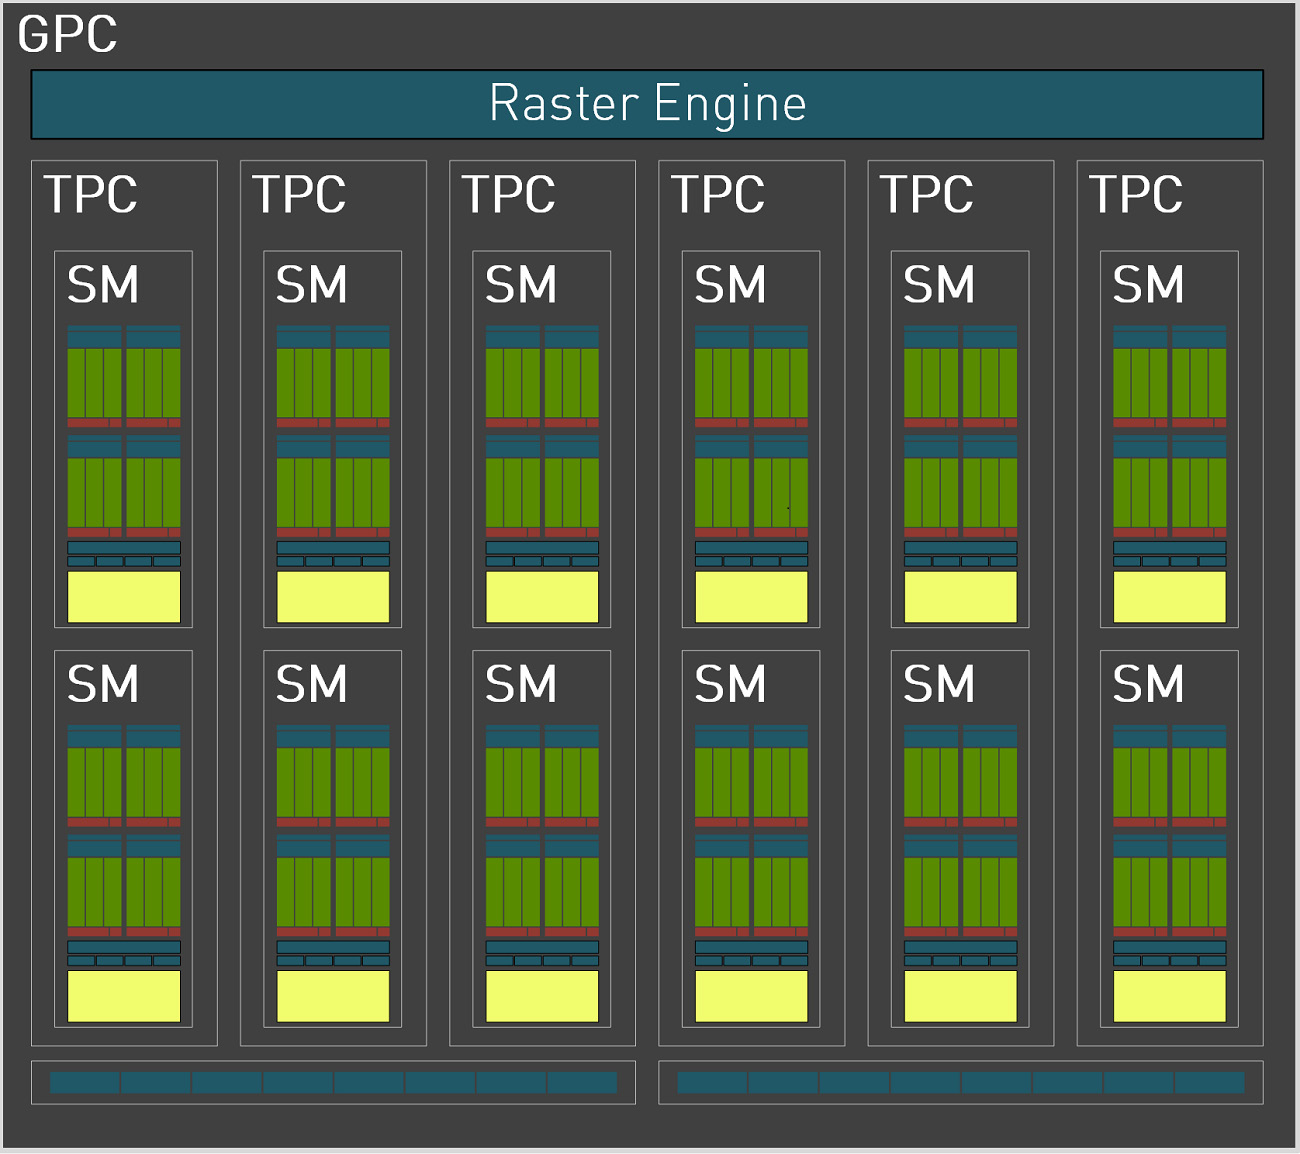
\includegraphics[width=0.54\textwidth]{Figures/GPU_Arch/AD102GPCDesign.png}
  \hfill
  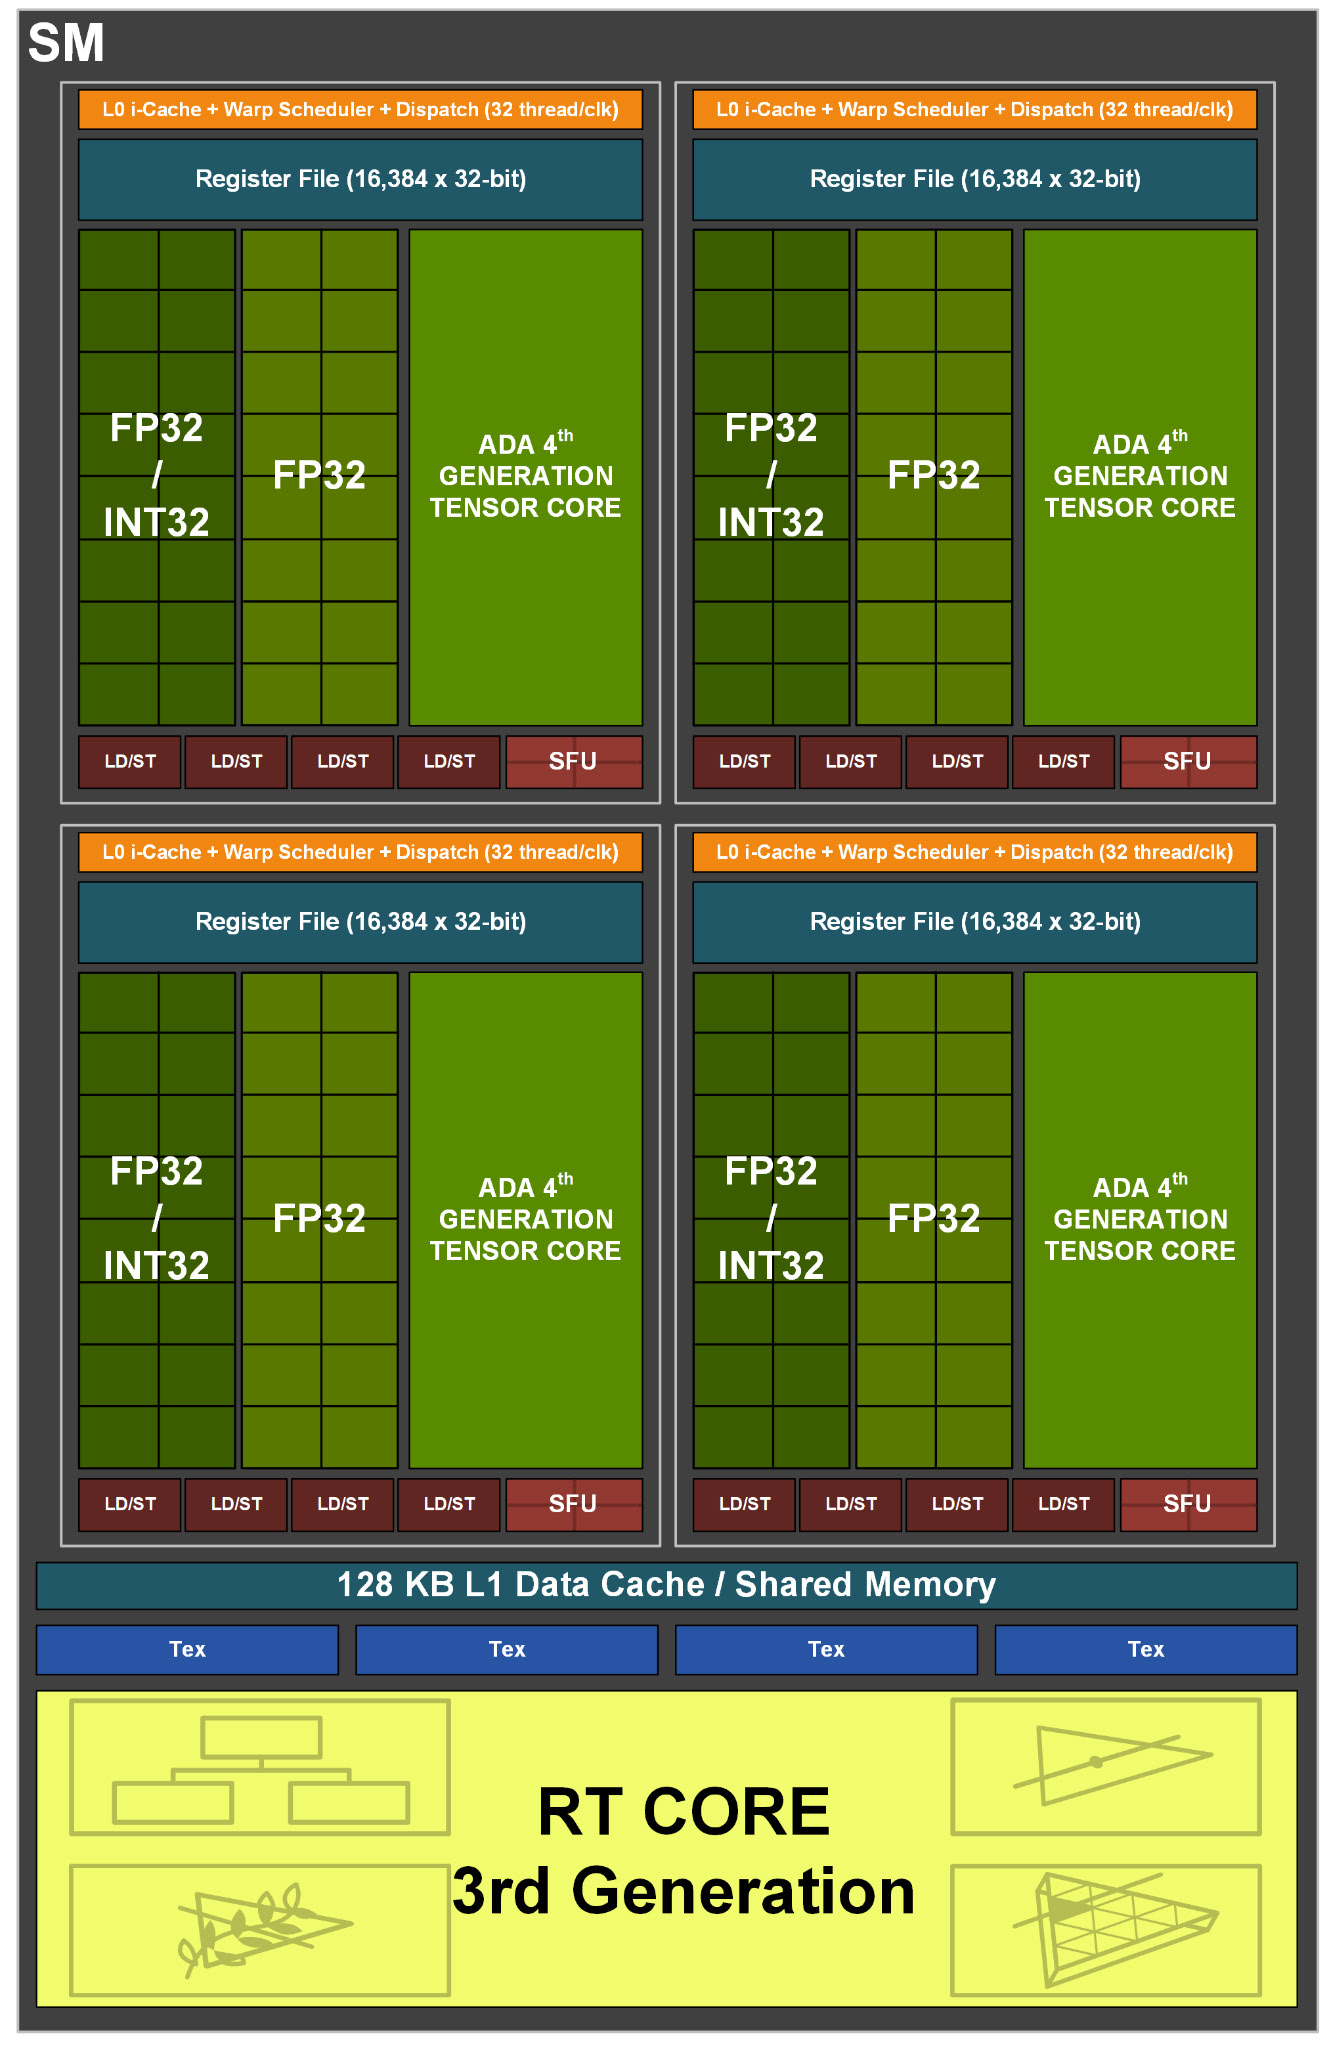
\includegraphics[width=0.32\textwidth]{Figures/GPU_Arch/AD102SMDesign.png}
  \end{subcaptiongroup}
  \bicaption{NVIDIA Ada Lovelace（AD102）GPU 架构层次\cite{nvidiaAdaGPUArchitecture2022}}{NVIDIA Ada Lovelace (AD102) GPU architecture hierarchy\cite{nvidiaAdaGPUArchitecture2022}}
  \label{fig:gpu_sm_rtcore}

  \small
  全芯片（上）、GPC（左下）与 SM（右下）。
  AD102 全芯片含 12 个 GPC、L2 Cache 及显存控制器；每个 GPC 包含 6 个 TPC，
  各 TPC 下辖 2 个 SM；每个 SM 含 4 个 Warp Scheduler、FP32/INT32 CUDA Core、
  第四代 Tensor Core 及底部的第三代 RT Core。
  RT Core 独立于 CUDA Core 执行 BVH 遍历与光线—三角形求交，
  SM 在 Warp 等待 RT Core 返回期间可调度其他就绪 Warp 继续计算。
\end{figure}

\subsection{本文涉及的几何查询类型}
%% 写作思路：
%%   - 说明热输运求解所需的几何查询并非只有标准"最近命中"光追，还需要另外两类特殊查询，
%%     这是第四章后端管线设计的直接需求来源。
%%   - 三类查询：
%%       (1) 最近命中光追（Closest-Hit）：沿光线方向找到第一个交点，用于辐射路径传播（主要查询）。
%%       (2) 最近面投影（Closest Point Projection，CP 查询）：给定空间点 $\mathbf{x}$，求
%%           场景表面上距其最近的三角形面片及精确投影位置——用于传导段 CND 布朗游走粒子的步长
%%           确定（距边界最近距离）和到达边界时触发 BND 事件。
%%           实现方式（基于 RTNN / PPoPP 2022）：将每个三角形预处理为以搜索半径膨胀的 AABB，
%%           查询点以"零长射线"（tmin=0, tmax=1e-16）发出，OptiX BVH 遍历找到所有含查询点的
%%           AABB，自定义 Intersection 程序以 Voronoi 区域法（双精度）计算到三角形精确距离，
%%           Payload 寄存器保留最近命中，输出距离、投影坐标、法向、面片索引。
%%       (3) 封闭腔体归属查询（Point-in-Enclosure，ENC 查询）：判断空间点是否位于某封闭腔体
%%           内部——用于确定给定位置的腔体归属（影响辐射边界条件的选取）。
%%           实现方式（两步）：
%%             Step 1: 对查询点执行 CP 查询，得到最近面片及其几何法向 $\hat{n}$；
%%             Step 2: 从查询点沿 $+X$ 方向发射单条标准 Closest-Hit 射线，读取命中法向 $\hat{n}_{\rm hit}$：
%%               射线未命中 → 外部（side=0）；
%%               命中：$\hat{n}_{\rm hit}.x < 0$ → 命中正面（外部，side=0）；
%%                      $\hat{n}_{\rm hit}.x > 0$ → 命中背面（内部，side=1）。
%%           即：法向点乘判侧，而非奇偶计数；使用标准 Closest-Hit 管线，非 Any-Hit。
%%   - 这三类查询将在第四章分别设计独立的 OptiX 管线（Pipeline）。
%% [引用需求] \cite{parkerOptiXGeneralPurpose2010}

由第 2.2 节与第 2.3 节的分析可知，耦合热输运路径追踪求解器所需的几何查询并非单一的标准最近命中光追，而是涵盖三类在物理语义上不同的查询，分别驱动路径状态机中的不同物理过程。这三类查询在第四章将各自设计独立的 OptiX 管线。

\textbf{第一类：最近命中光追（Closest-Hit Ray Tracing，RT 查询）。} 给定光线起点 $\mathbf{o}$ 与方向 $\hat{\mathbf{d}}$，在场景三角形网格中求第一个几何交点 $(\mathbf{x}^*, \hat{n}^*)$ 及对应的表面属性（材质编号、封闭腔体归属、发射率等）。该查询驱动 RAD 辐射、BND 各类界面步骤及 CND 传导步中凡涉及直接射线求交的过程，均向 RT 挂起队列提交请求，是三类查询中批量规模最大的一类，也是 OptiX/RT Core 最直接支持的查询类型。

\textbf{第二类：最近面投影（Closest Point Projection，CP 查询）。} 给定空间中任意点 $\mathbf{x}$，求场景表面上距其欧氏距离最小的点 $\mathbf{x}^* = \arg\min_{\mathbf{y} \in \partial\Omega}\|\mathbf{y} - \mathbf{x}\|$ 及其表面法向 $\hat{n}^*$。该查询仅用于传导段（CND）Walk-on-Spheres（WoS）游走路径变体的步长计算——WoS 算法需要当前位置至场景表面的最近距离来确定每步游走的球半径，并在粒子进入 epsilon-shell 时触发 BND 界面事件。

\textbf{第三类：封闭腔体归属查询（Point-in-Enclosure，ENC 查询）。} 给定空间中任意点 $\mathbf{x}$，判断其归属于哪个封闭腔体（Enclosure）。封闭腔体是 Stardis 场景模型的基本组织单元，每个腔体对应一组闭合固体表面，辐射边界条件的选取依赖于路径当前所处腔体的编号。ENC 查询通过向场景发射多条探测射线并依据命中面法向判侧来确定归属关系，主要用于 BND 界面事件中的腔体归属判断。

三类查询的语义、驱动过程与实现方案如表\,\ref{tab:query_types} 所示：

\begin{table}[htbp]
    \centering
    \bicaption{耦合热输运求解器所需的三类几何查询}{Three geometric query types in the coupled heat transport solver}
    \label{tab:query_types}
    \begin{tabular}{llll}
        \toprule
        查询类型 & 缩写 & 驱动过程 & 实现方式 \\
        \midrule
        最近命中光追 & RT & 各过程直接射线求交 & OptiX Closest-Hit 管线 \\
        最近面投影 & CP & CND 游走步长计算 & 场景表面最近点批量查询 \\
        封闭腔体归属查询 & ENC & BND 腔体归属判断 & 多方向探测射线 $+$ 法向判侧 \\
        \bottomrule
    \end{tabular}
\end{table}

\paragraph{建模假设与适用边界。}为聚焦于求解架构的并行化设计，本文蒙特卡洛耦合热输运框架采用三条工程简化假设，其在主流工业红外仿真任务中通常成立：（1）漫射灰体表面，即发射率与吸收率独立于波长且与方向无关；（2）透明非参与流体，即流体仅承担对流换热，不参与体积辐射散射或吸收；（3）线性化对流换热系数，即对流换热在工程温区内以恒定或弱温度依赖系数近似。上述假设的失效场景及对应扩展路径将在第六章展望中讨论。

\section{本章小结}

本章系统梳理了支撑本文工作的核心理论与技术基础。

第 2.1 节建立了耦合热输运的物理模型：分别阐述热传导、热辐射与热对流三种基本传热机制的物理规律及数学描述，并以联合能量平衡边界条件统一刻画三种机制在固-流界面处的耦合关系。其中热传导作为三维抛物型偏微分方程，以体积随机游走形式参与蒙特卡洛求解，几何查询开销远超其他过程，是驱动 GPU 硬件光追加速的核心动机。

第 2.2 节阐述了蒙特卡洛路径追踪在耦合热输运中的应用原理：从蒙特卡洛积分的基础理论出发，回顾经典正向追踪与反向路径追踪范式，重点介绍 Bati 等人将辐射、传导、对流三种机制统一至单一路径空间的耦合估计量框架，并以原始递归求解器实现为基准，指出其在批量化方面的结构性局限。

第 2.3 节与第 2.4 节分别介绍了两大工程技术基础。Wavefront 执行模型通过引入持久化路径状态与挂起队列，将状态推进与几何查询执行解耦，使大批量几何查询在架构层面成为可能，为第三章并行化求解器的设计提供范式依据。光线追踪与几何查询加速技术系统介绍了水密求交算法、BVH 层次加速结构，以及 Intel Embree（CPU 基准后端）与 NVIDIA OptiX/RT Core（GPU 硬件光追后端）两条工程路线，并明确了耦合热输运求解器所需的三类几何查询（RT、CP、ENC），为第四章 OptiX 后端三条管线的设计奠定直接基础。